
In this analysis we use a definition of d0 that is relative to the beam line, and additionally correct for some global biases due to mis-alignment in the data only based on the year and period that the data is taken.
% These choices are explained in this section.

% \subsection{Beam Line} % vs Primary Vertex Reference Frame
% \label{sec:d0_beamLineVsprimaryVertex}

% By default in the ATLAS software d0 is defined with respect to the beam line. This gives a global reference frame for which it can be defined for any vertex, and for events without any primary vertex. 
% In this analysis we keep this reference frame such that muons in our control selection of $Z \rightarrow \mu\mu$ events have identical resolution to those in our signal $W$ selection. 
% In this section we briefly discuss this choice and alternatives.

\subsection{Alignment Corrections}
\label{sec:corrections}

% \begin{figure}[htbp]
% \centering
% \subfloat[Data 2017]{{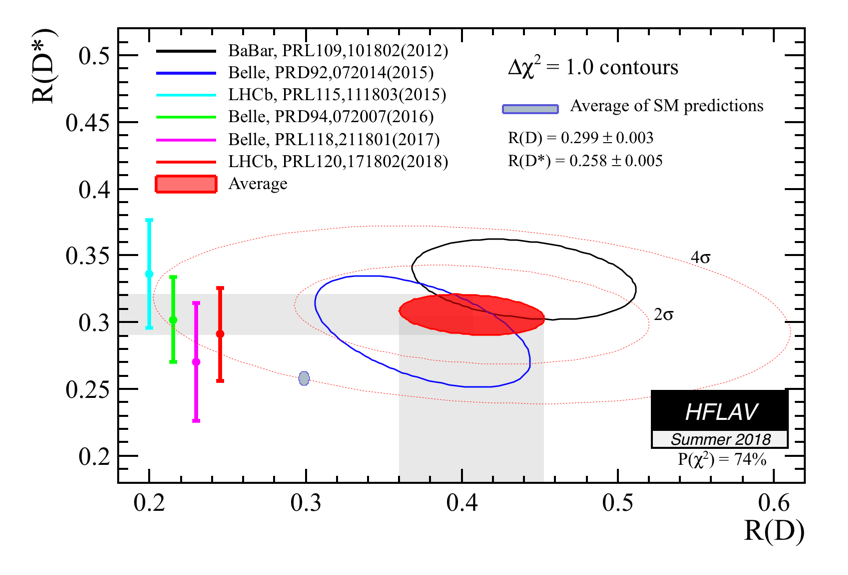
\includegraphics[width=0.45\textwidth]{figures/intro/rdrds_summer18.png} }}
% \subfloat[Data 2018]{{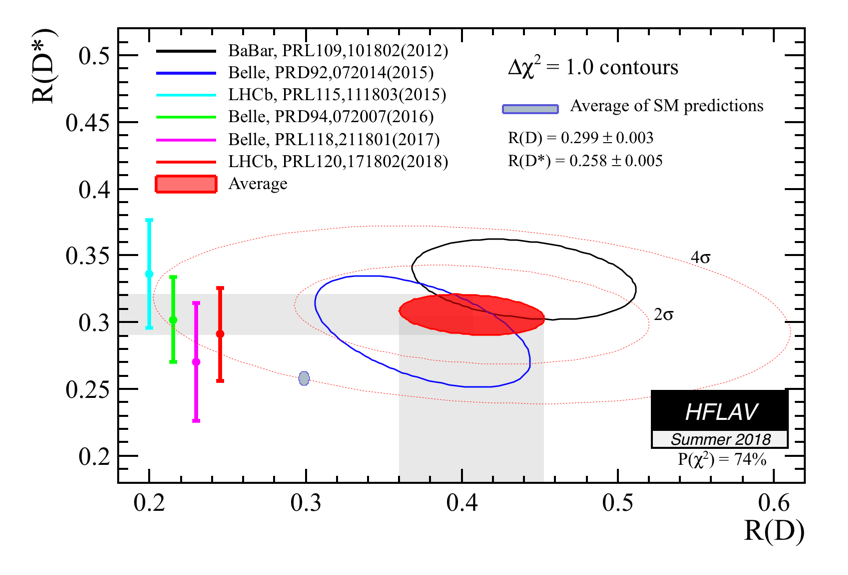
\includegraphics[width=0.45\textwidth]{figures/intro/rdrds_summer18.png} }}
% \caption{
%   The $d_0$ distribution for probe muons in 2017 (blue) and 2018 (red) data in the $Z$ control selection. 
%   Gaussian fits are performed to determine any global mis-alignment and the resolution. 
%   Good alignment is seen in both datasets with sub-micro offsets from zero and there is reasonable agreement between the years in the resolution. 
%   This shows that the lack of re-processing of the 2018 data does not cause significant issues for this analysis.
% }
% \label{fig:d0_2017_2018}
% \end{figure}

% The inner detector tracking group ensures that the detector is properly aligned in the data. 
% The 2018 data has not been reprocessed as the alignment was deemed good enough for analyses based on the 2017 conditions. 
% Figure \ref{fig:d0_2017_2018} shows that the 2017 and 2018 data appear to have sub-micron offsets in $d_0$ such that any correction to re-center these distributions would not significantly improve the resolution. 
% Additionally the resolution of $d_0$ is very similar between the years indicating that the lack of re-processing of 2018 data is not a large issue for this analysis.

% After re-processing of the data there can remain residual imperfections in the alignment. 
% These can results in charge dependent or charge independent biases in the $d_0$ distribution. 
The time dependent, charge independent, bias of the $d_0$ distribution is shown in Fig.\ref{fig:d0_bias_per_years}. 
Clearly in 2015 
% and 2016 
there remains a significant bias.
% , while in 2017 and 2018 data the biases are small. 
Therefore in the analysis we correct $d_0$ using a simple charge independent shift in the $d_0$ value:
\begin{equation}
  \label{eq:d0bias}
  d_0^{'} = d_0 - \alpha
\end{equation}
for 2015 data where $\alpha = -0.004479 \pm 0.000013$ mm.
% , 2016 data in periods A+B (\todo{$\alpha = XX(\pm XX)$} mm), and the remainder of 2016 data (\todo{$\alpha = XX(\pm XX)$} mm).
We additionally check that these corrections are appropriate for all $p_T$, $\eta$, and $\varphi$ in \ref{fig:d0_bias_eat_pt} and see that the same correction can be applied independent of momentum and position.

These corrections to the 2015 data 
% and 2016 
are in agreement with corrections obtained by the Top group in the $t\bar{t}$ analysis \cite{Mcfayden:2667199} and are applied in the remainder of this analysis.

\begin{figure}[htbp]
\centering
\subfloat[2015 Data]{{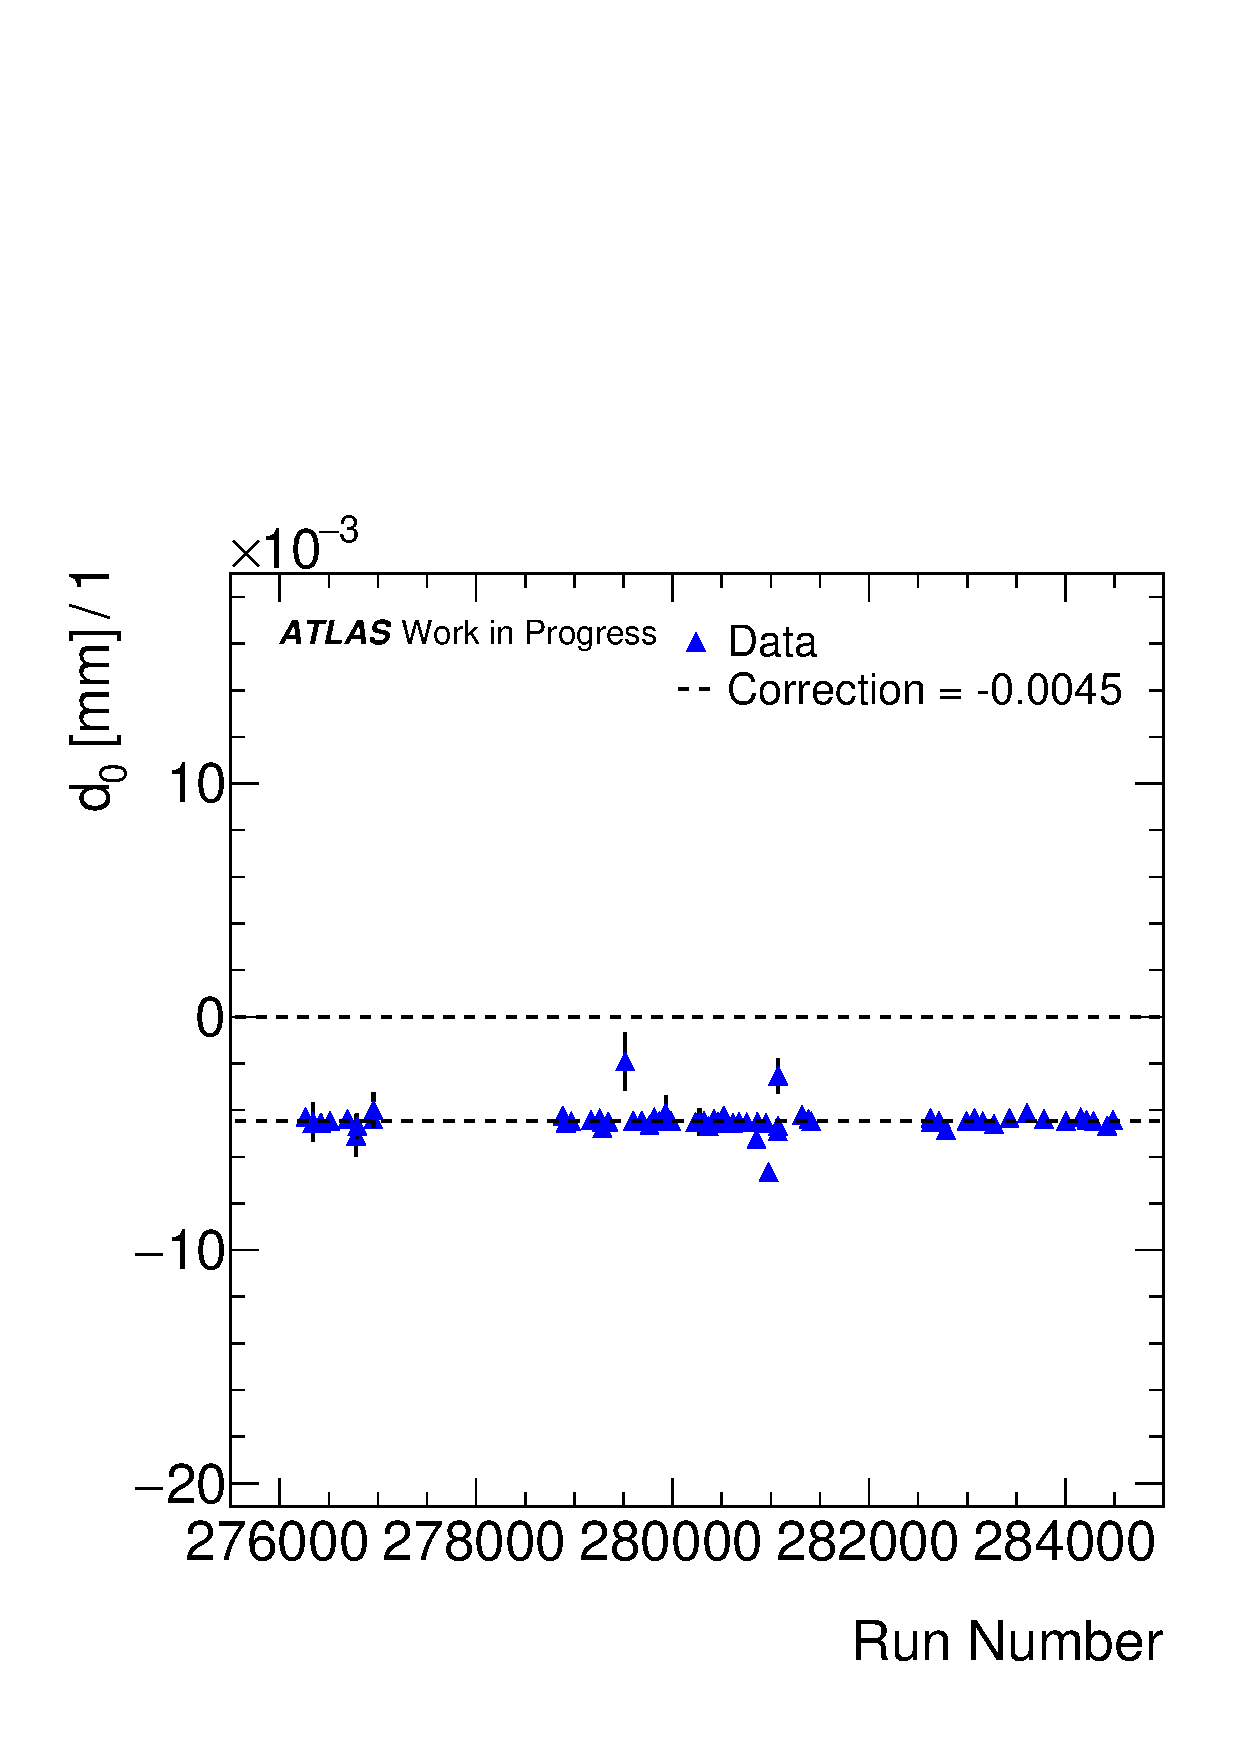
\includegraphics[width=0.45\textwidth]{figures/d0_bias/profile_lep_0_trk_d0_vs_RunNumber15-ZR-mu.pdf} }}
% \subfloat[2016 Data]{{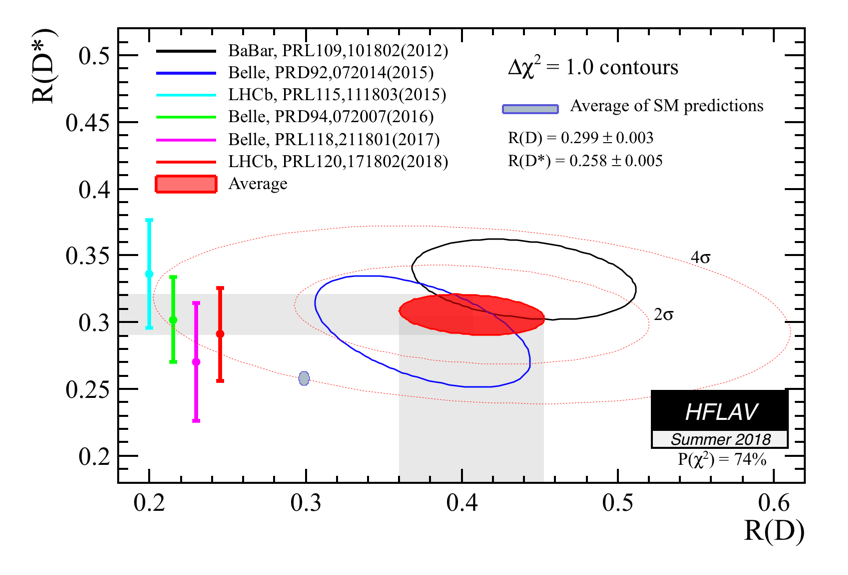
\includegraphics[width=0.45\textwidth]{figures/intro/rdrds_summer18.png} }}
% \\
% \subfloat[2017 Data]{{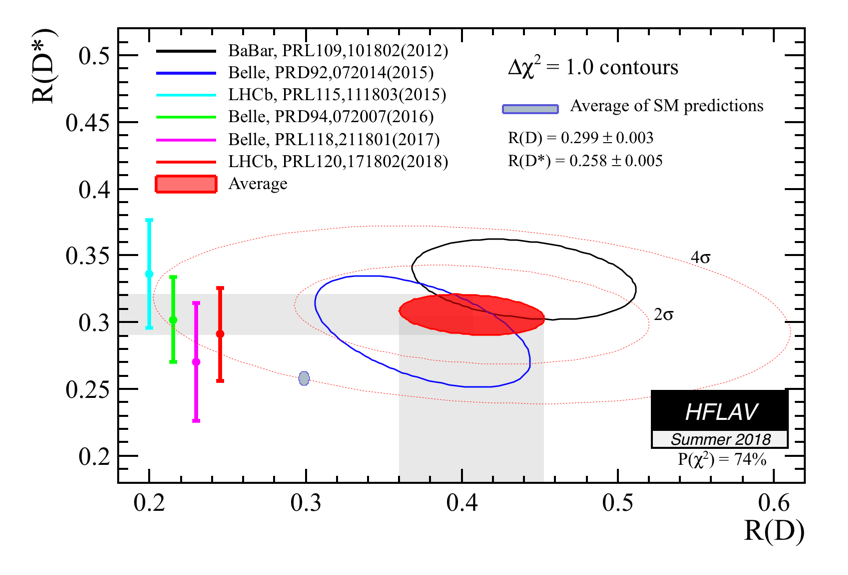
\includegraphics[width=0.45\textwidth]{figures/intro/rdrds_summer18.png} }}
% \subfloat[2018 Data]{{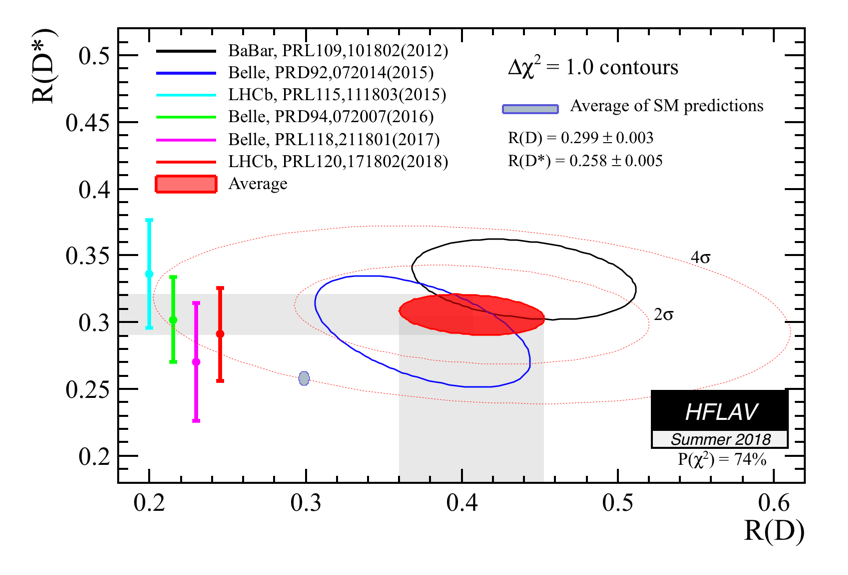
\includegraphics[width=0.45\textwidth]{figures/intro/rdrds_summer18.png} }}
\caption{
  The average $d_0$ of leading leptons in $Z \rightarrow \mu\mu$ selection across 2015 year
%   different years 
  by RunNumber.
  The 
%   biases in 2017 and 2018 are very small but 
  significant biases relative to the resolution are seen in 2015 
%   and 2016 
  which we correct for.
}
\label{fig:d0_bias_per_years}
\end{figure}


\begin{figure}[htbp]
\centering
\subfloat[$\eta$ 2015]{{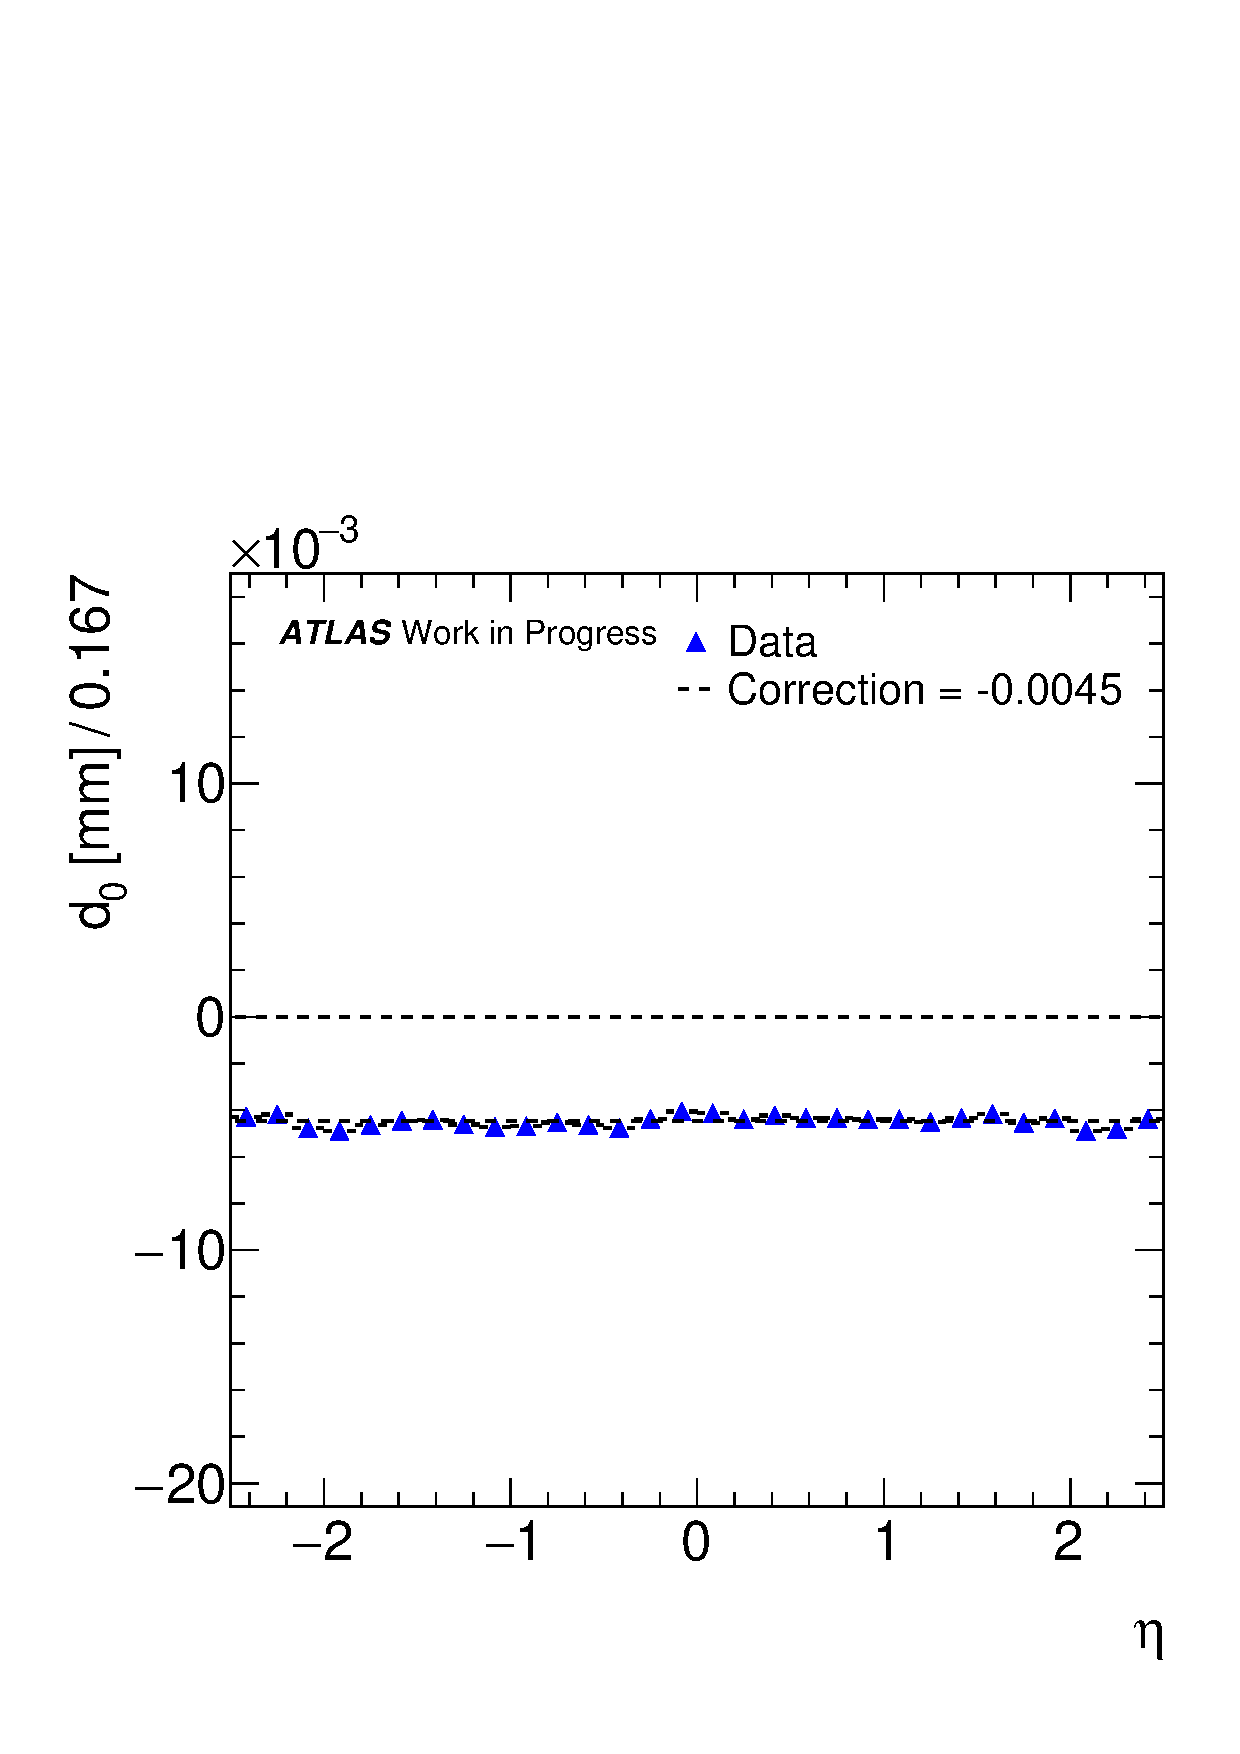
\includegraphics[width=0.31\textwidth]{figures/d0_bias/profile_lep_0_trk_d0_vs_lep_0_eta-ZR-mu.pdf} }}
\subfloat[$\varphi$ 2015]{{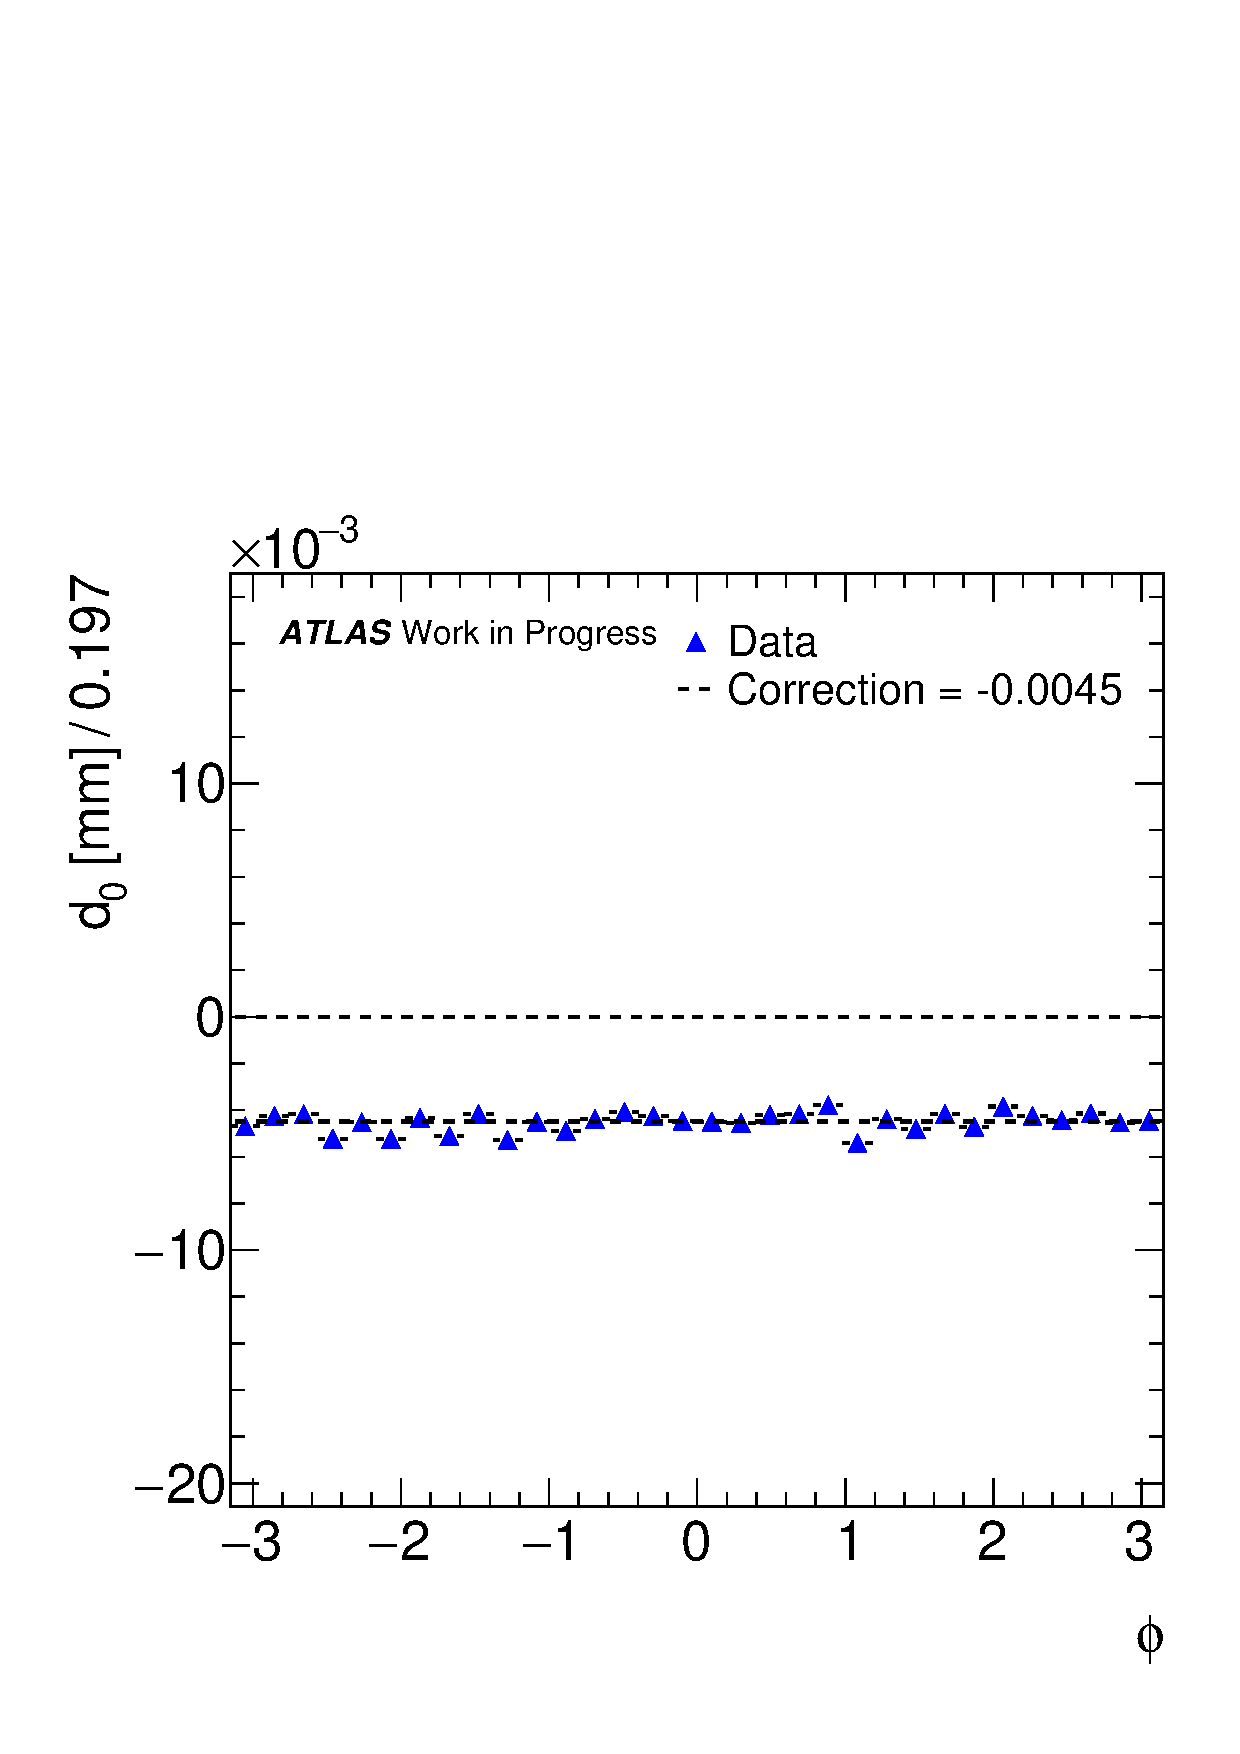
\includegraphics[width=0.31\textwidth]{figures/d0_bias/profile_lep_0_trk_d0_vs_lep_0_phi-ZR-mu.pdf} }}
\subfloat[$p_T$ 2015]{{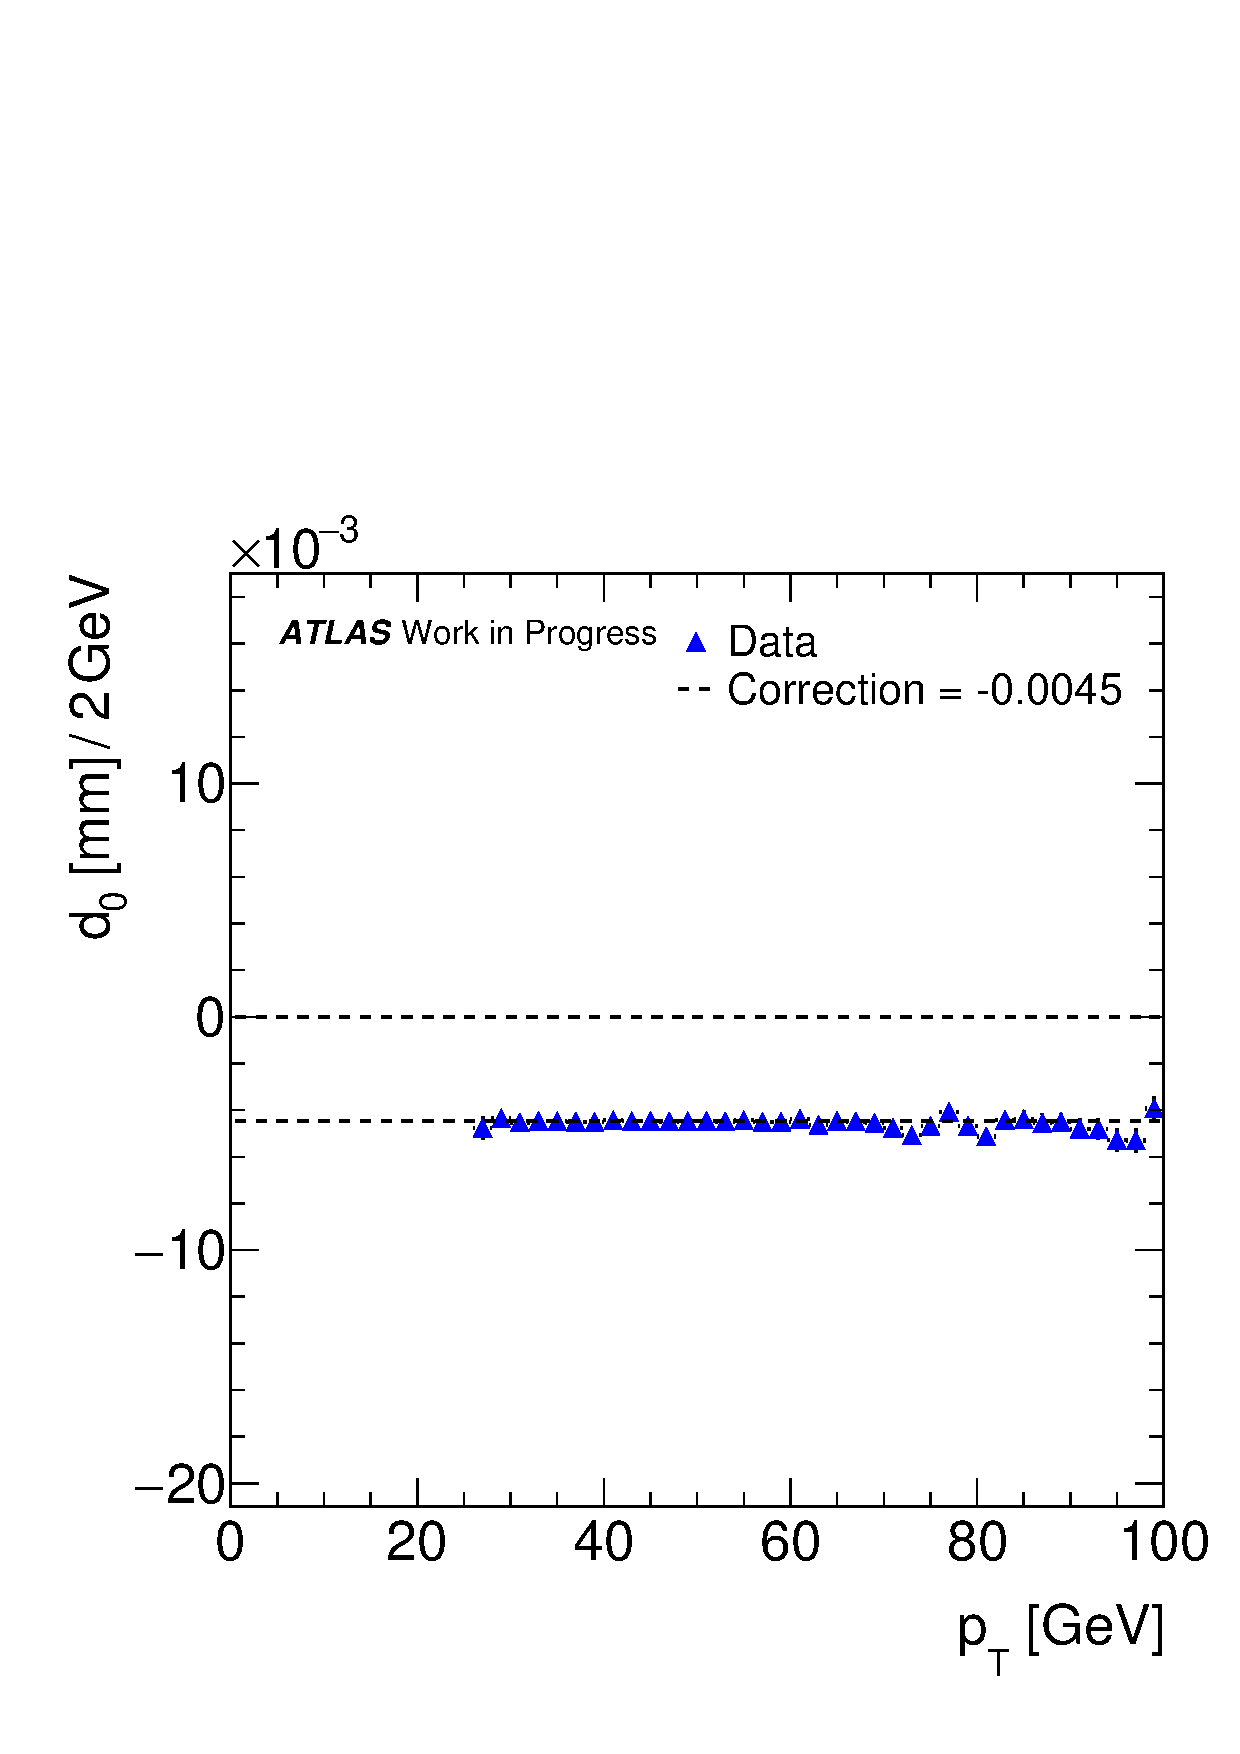
\includegraphics[width=0.31\textwidth]{figures/d0_bias/profile_lep_0_trk_d0_vs_lep_0_pt-ZR-mu.pdf} }}
% \\
% \subfloat[$\eta$ 2016AB]{{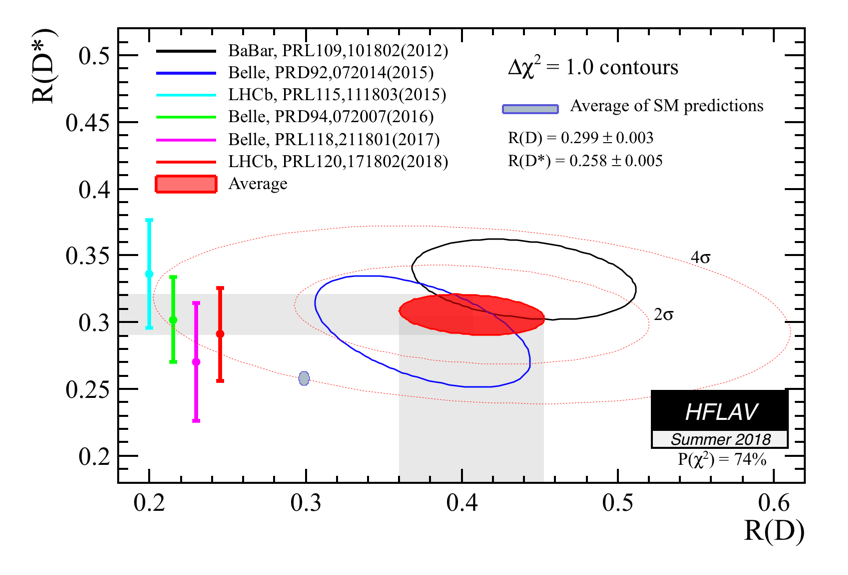
\includegraphics[width=0.31\textwidth]{figures/intro/rdrds_summer18.png} }}
% \subfloat[$\varphi$ 2016AB]{{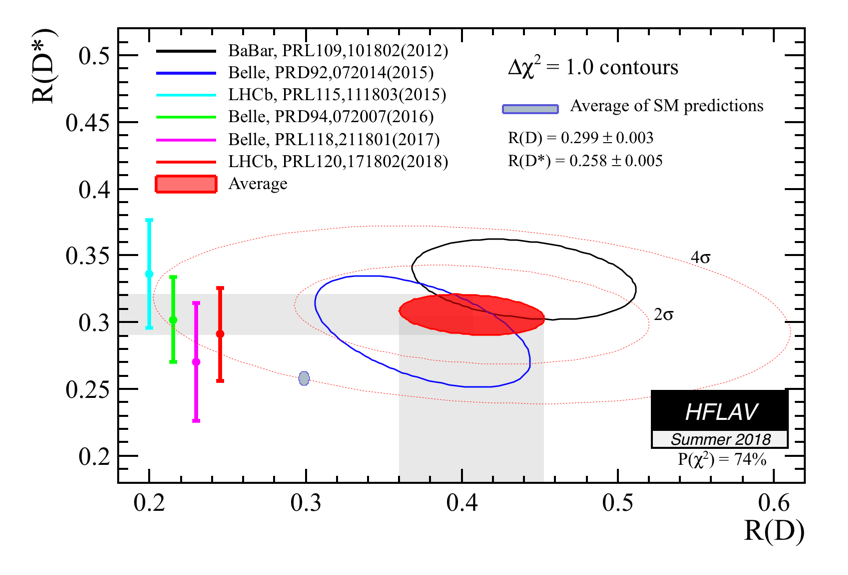
\includegraphics[width=0.31\textwidth]{figures/intro/rdrds_summer18.png} }}
% \subfloat[$p_T$ 2016AB]{{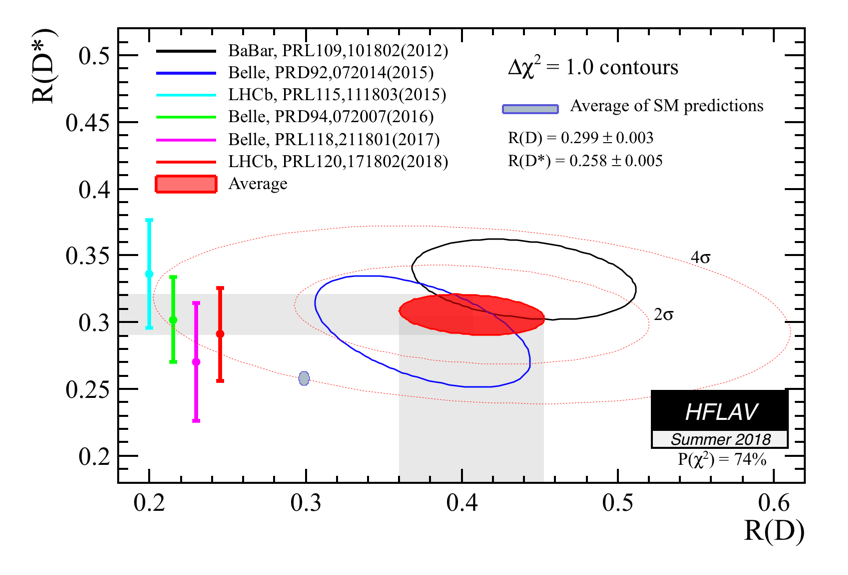
\includegraphics[width=0.31\textwidth]{figures/intro/rdrds_summer18.png} }}
% \\
% \subfloat[$\eta$ 2016Cp]{{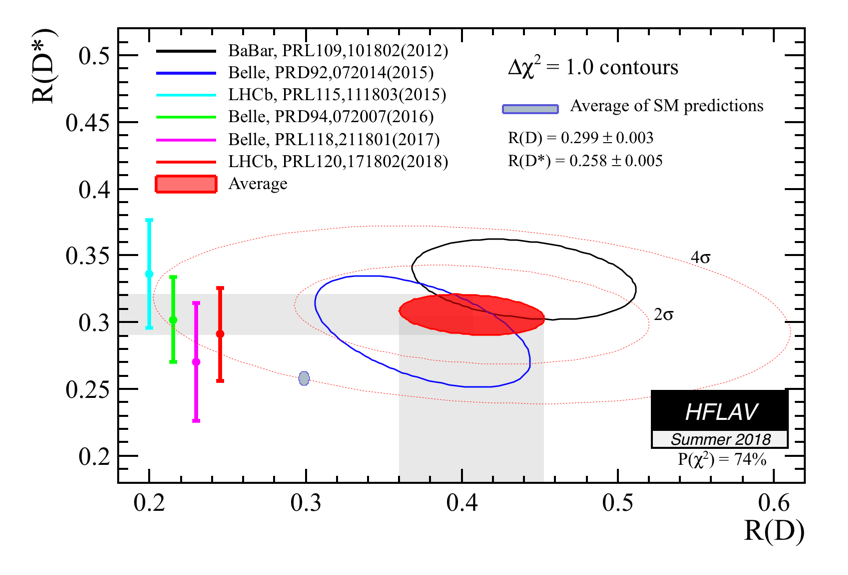
\includegraphics[width=0.31\textwidth]{figures/intro/rdrds_summer18.png} }}
% \subfloat[$\varphi$ 2016Cp]{{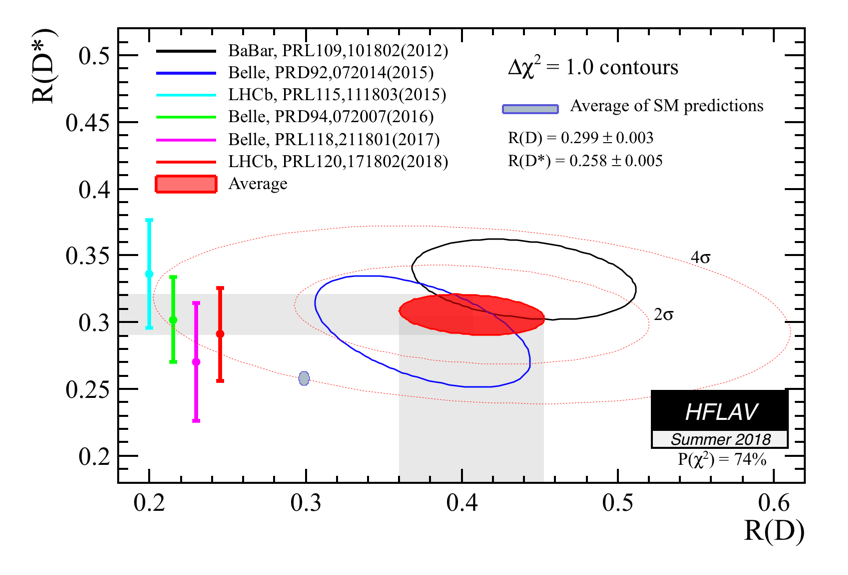
\includegraphics[width=0.31\textwidth]{figures/intro/rdrds_summer18.png} }}
% \subfloat[$p_T$ 2016Cp]{{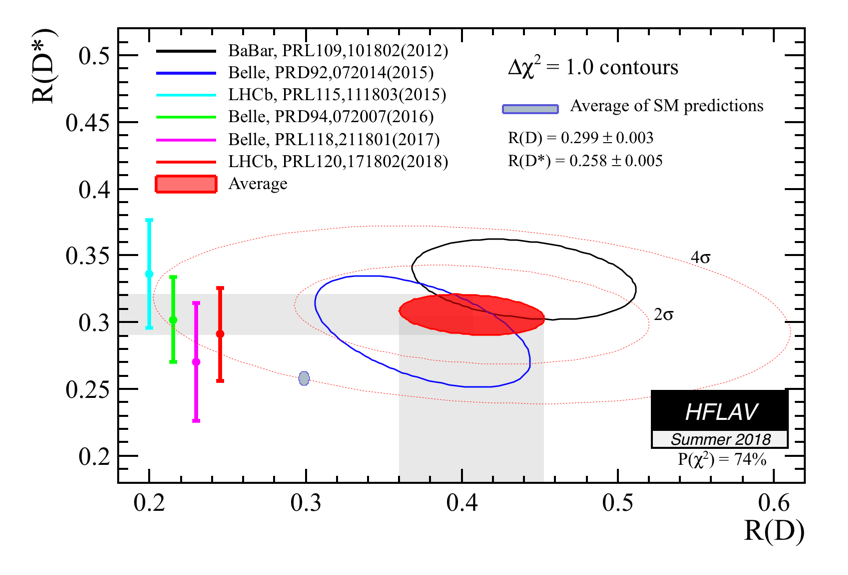
\includegraphics[width=0.31\textwidth]{figures/intro/rdrds_summer18.png} }}
% \\
% \subfloat[$\eta$ 2017]{{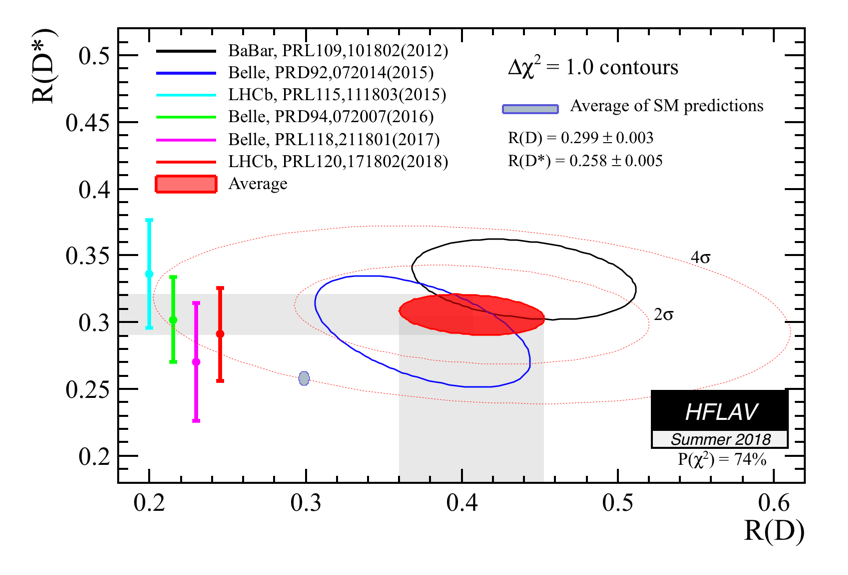
\includegraphics[width=0.31\textwidth]{figures/intro/rdrds_summer18.png} }}
% \subfloat[$\varphi$ 2017]{{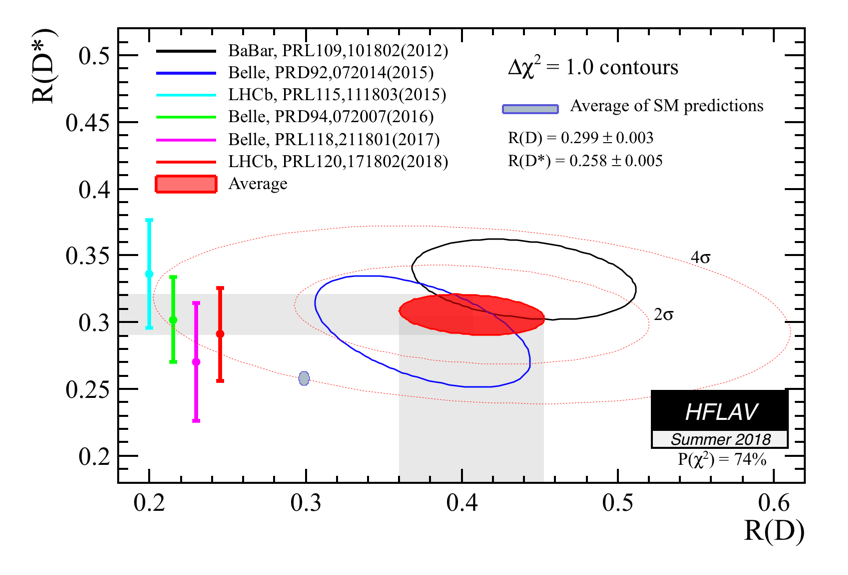
\includegraphics[width=0.31\textwidth]{figures/intro/rdrds_summer18.png} }}
% \subfloat[$p_T$ 2017]{{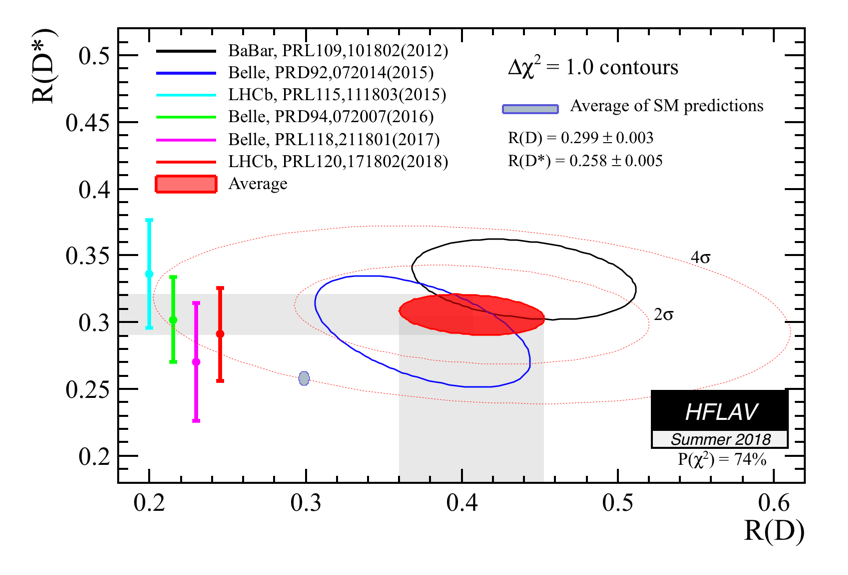
\includegraphics[width=0.31\textwidth]{figures/intro/rdrds_summer18.png} }}
% \\
% \subfloat[$\eta$ 2018]{{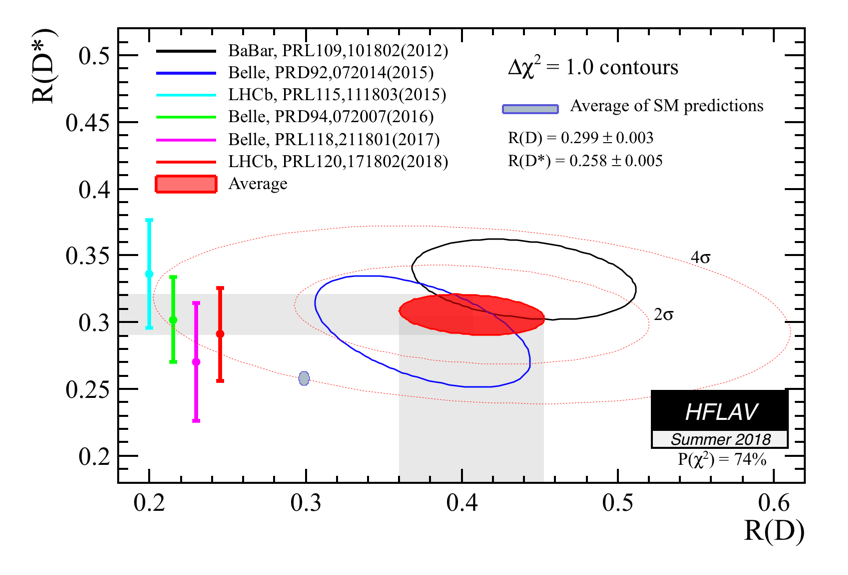
\includegraphics[width=0.31\textwidth]{figures/intro/rdrds_summer18.png} }}
% \subfloat[$\varphi$ 2018]{{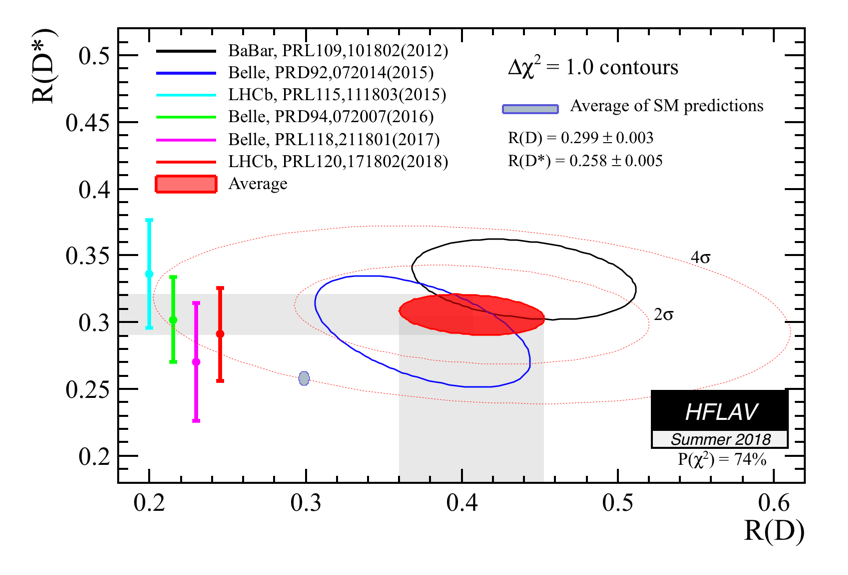
\includegraphics[width=0.31\textwidth]{figures/intro/rdrds_summer18.png} }}
% \subfloat[$p_T$ 2018]{{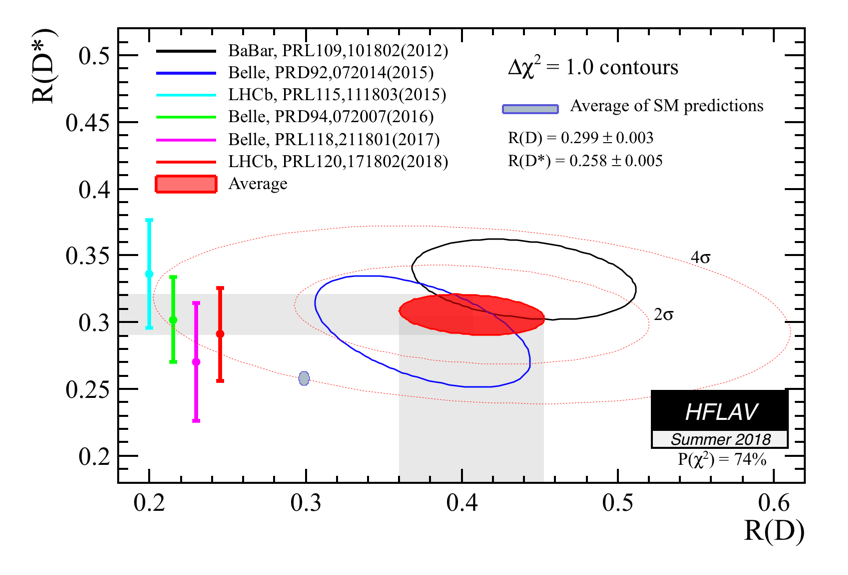
\includegraphics[width=0.31\textwidth]{figures/intro/rdrds_summer18.png} }}
\caption{
  The dependence on $p_T$, $\eta$, and $\varphi$ of the bias in $d_0$ of the probe lepton in $Z \rightarrow \mu\mu$ selection in 2015 year.
%   different years and periods.
}
\label{fig:d0_bias_eat_pt}
\end{figure}



\subsubsection{Calibration of impact parameter of prompt muons}
\label{sec:d0calibration_of_prompt_muons}

The calibration of $d_0$ distribution of prompt leptons is performed using $Z^{0}\rightarrow\mu^{+}\mu^{-}$ events. The selection of the calibration sample is same as described in Section~\ref{sec:z_boson_selection}.

We perform the calibration independently for each year of data taking.
The obtained samples contain mainly prompt leptons coming from $Z^{0}\rightarrow\mu^{+}\mu^{-}$ with a very small contamination from other sources.
The details on the origin of the tag lepton in the 2015 sample are shown on \ref{fig:Zmumu_mass_composition}.
The composition of the samples in other years is similar.
Hence, the impact of systematic uncertainties due to modelling of different processes on the calibration procedure is negligible.

\begin{figure}[htbp]
\centering
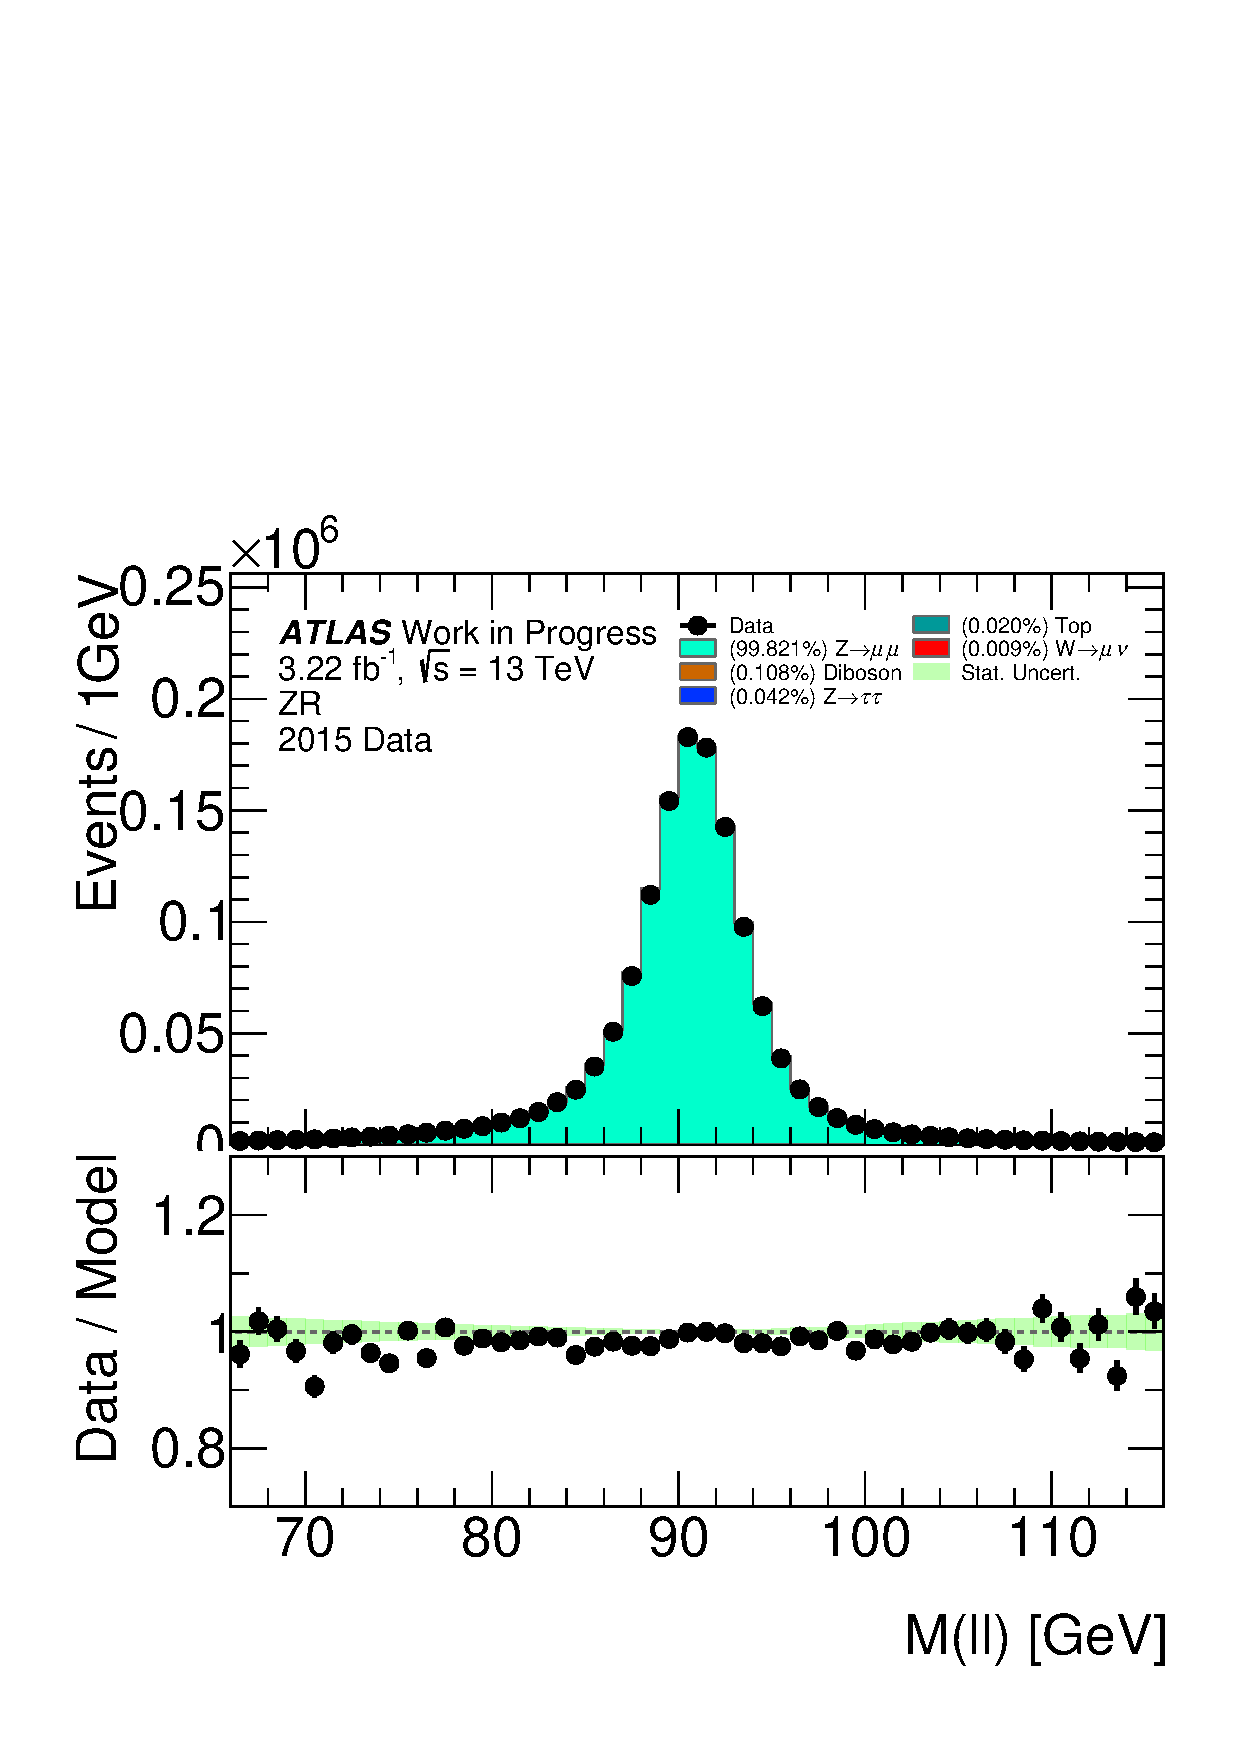
\includegraphics[width=0.45\textwidth]{figures/ZR/dataMc-dilep_m-ZR-mu.pdf}
\caption{
   Classification of the probe leptons in the 2015 $\mu^+\mu^-$ sample selected for $d_0$ calibration.
}
\label{fig:Zmumu_mass_composition}
\end{figure}

The $d_0$ distribution varies for different values of $p_T$ and $\eta$ of the leading lepton as demonstrated in Figures \ref{fig:d0_2015_pTDep} and \ref{fig:d0_2015_etaDep}. 
It can be seen that the dependence of d0 distribution on the lepton $p_T$ is strong.
The variation of the distributions with the change of $\eta$ is also visible.
Therefore, we determine the $d_0$ distribution separately in several kinematic bins depending on $p_T$ and $|\eta|$ of the leading lepton.

\begin{figure}[htbp]
\centering
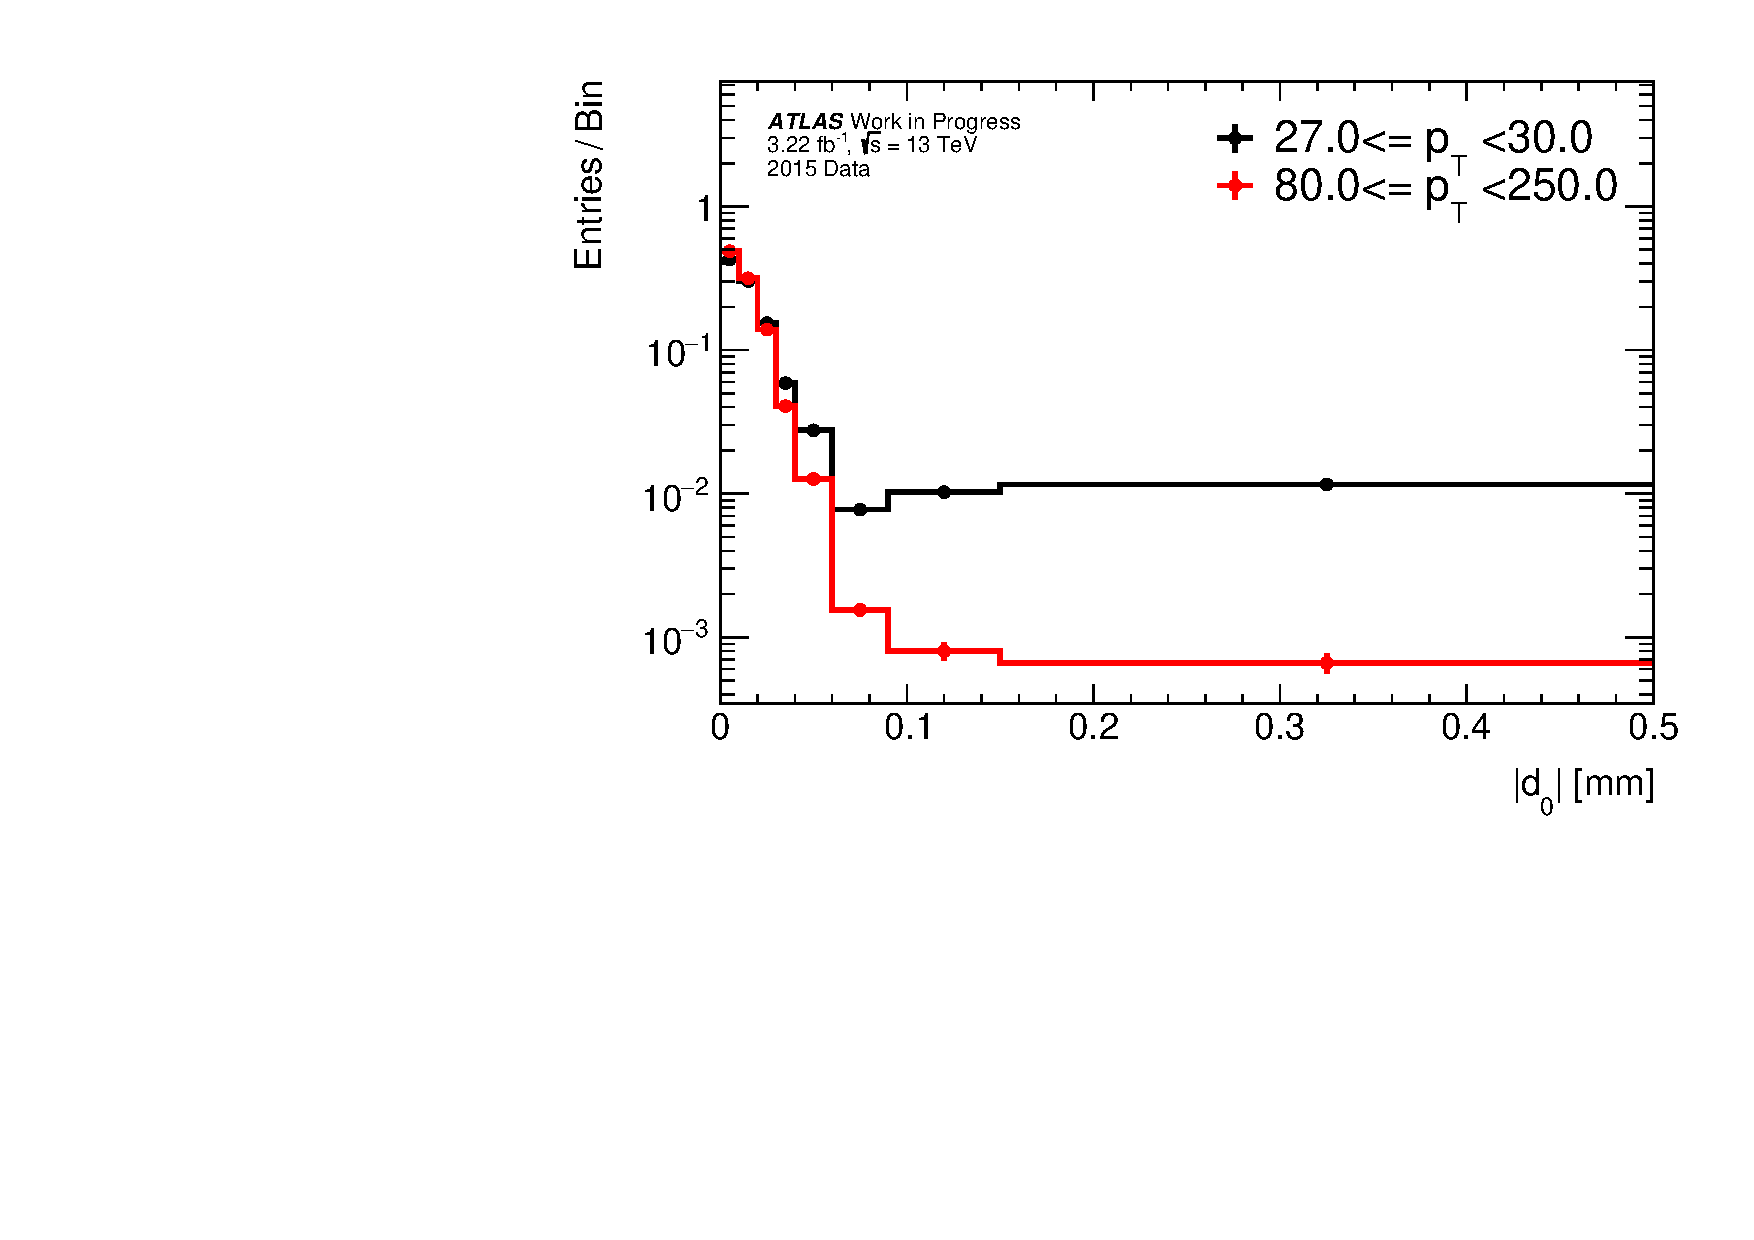
\includegraphics[width=0.45\textwidth]{figures/ZR/d0_smearing/twoplots_TwoPlots_pT-fit_fabs_lep_0_trk_d0_cor-SR-mu.pdf}
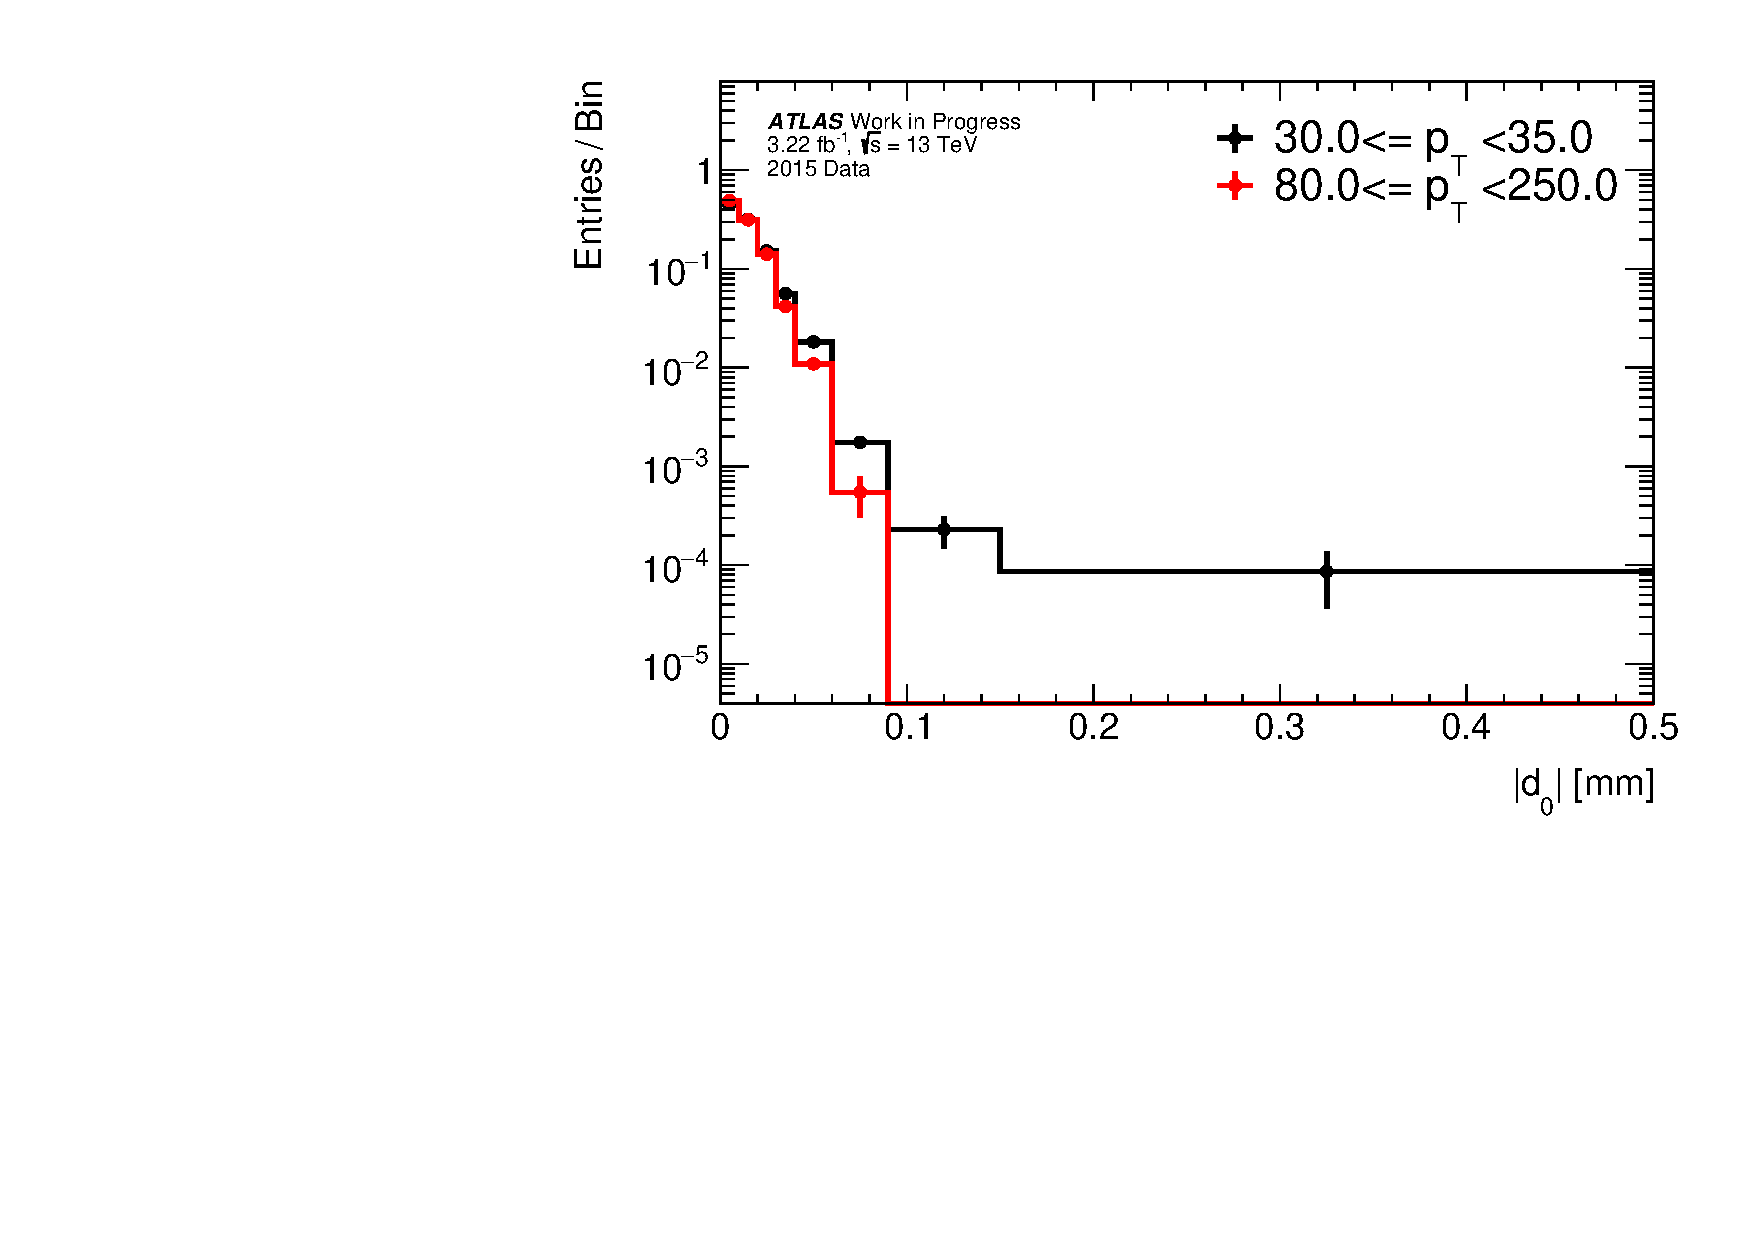
\includegraphics[width=0.45\textwidth]{figures/ZR/d0_smearing/twoplots_TwoPlots_pT-fit_fabs_lep_0_trk_d0_cor-ZR-mu.pdf}
\caption{
  Normalised $d_0$ distributions in data of muons with $30 < p_T < 35$ GeV and $80 < p_T < 250$ GeV.
  For all distributions muons with $0 < |\eta| < 0.8$ were used.
  Signal region (left) and $Z^{0}\rightarrow\mu^{+}\mu^{-}$ region (right).
}
\label{fig:d0_2015_pTDep}
\end{figure}

\begin{figure}[htbp]
\centering
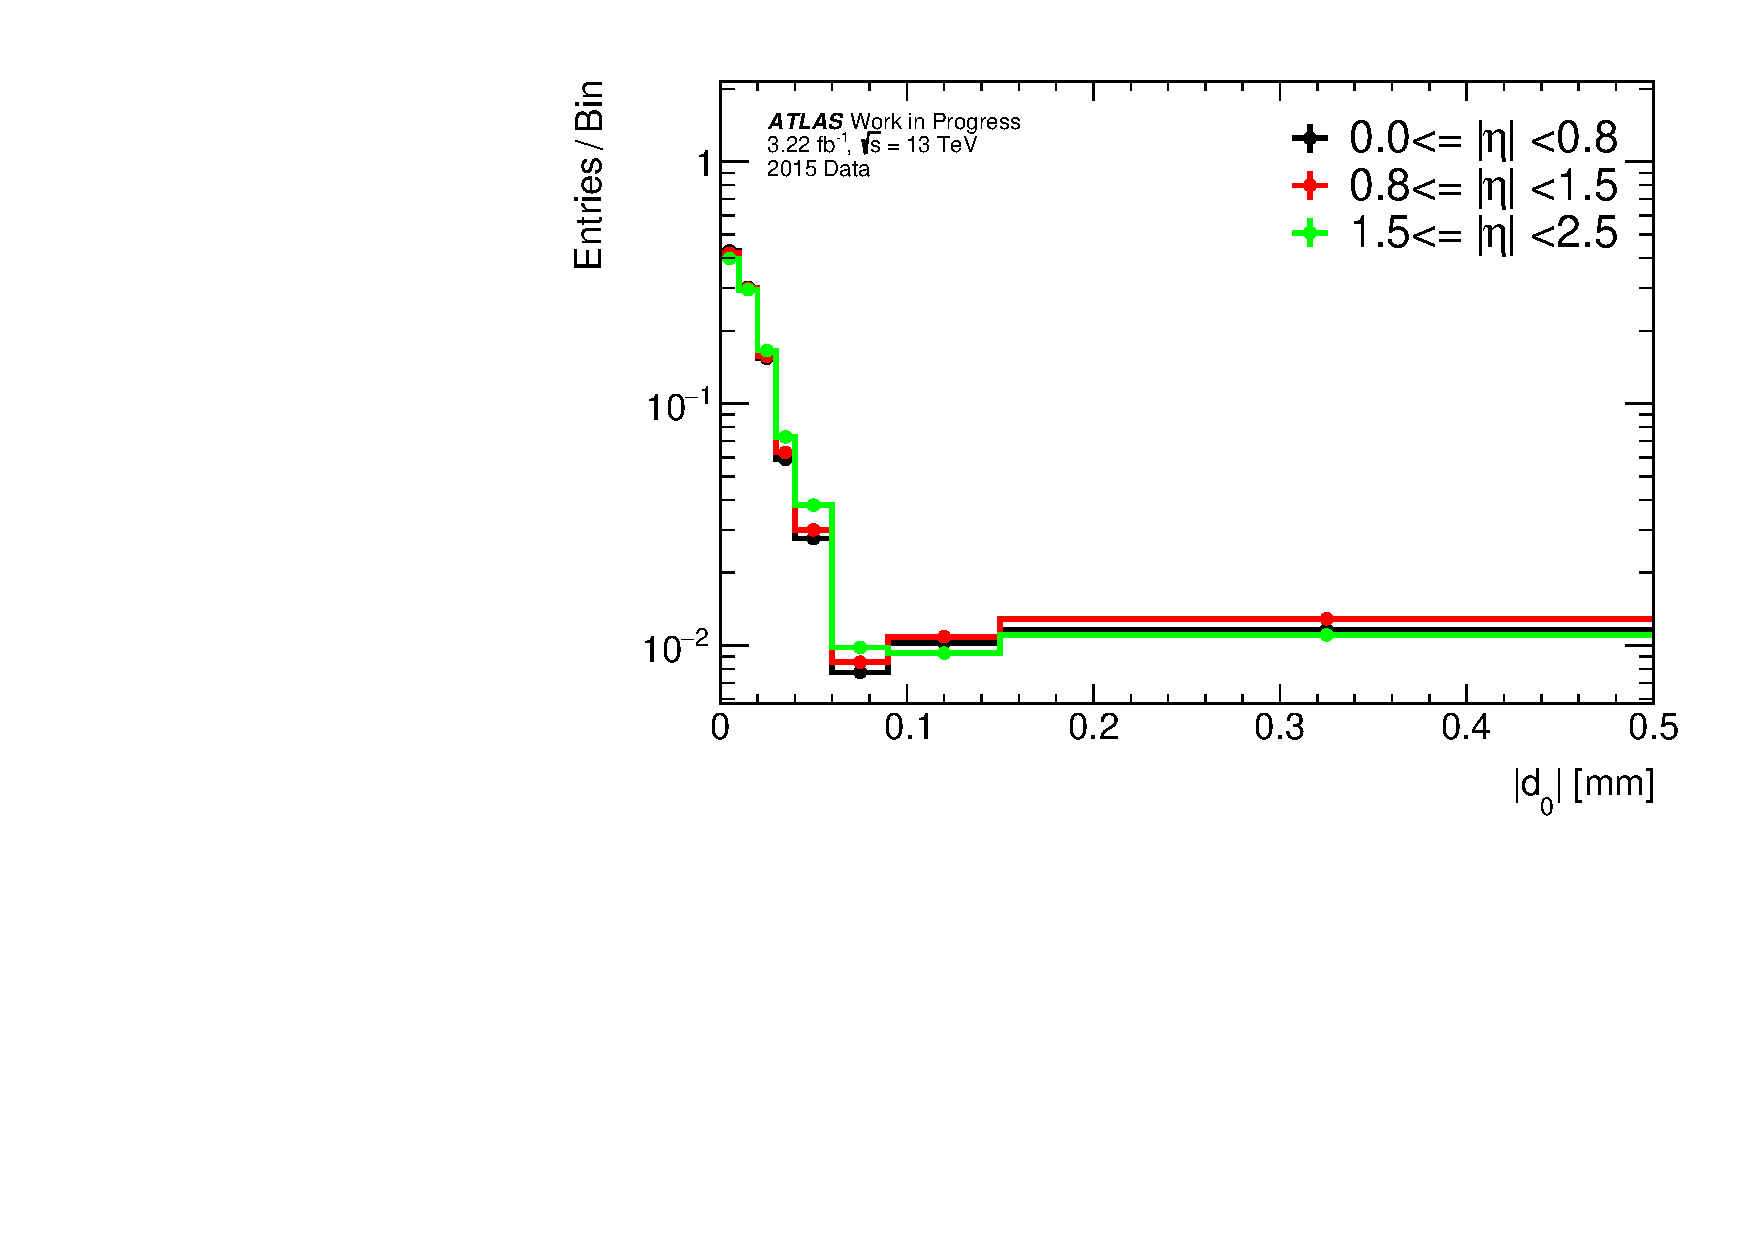
\includegraphics[width=0.45\textwidth]{figures/ZR/d0_smearing/twoplots_TwoPlots_eta-fit_fabs_lep_0_trk_d0_cor-SR-mu.pdf}
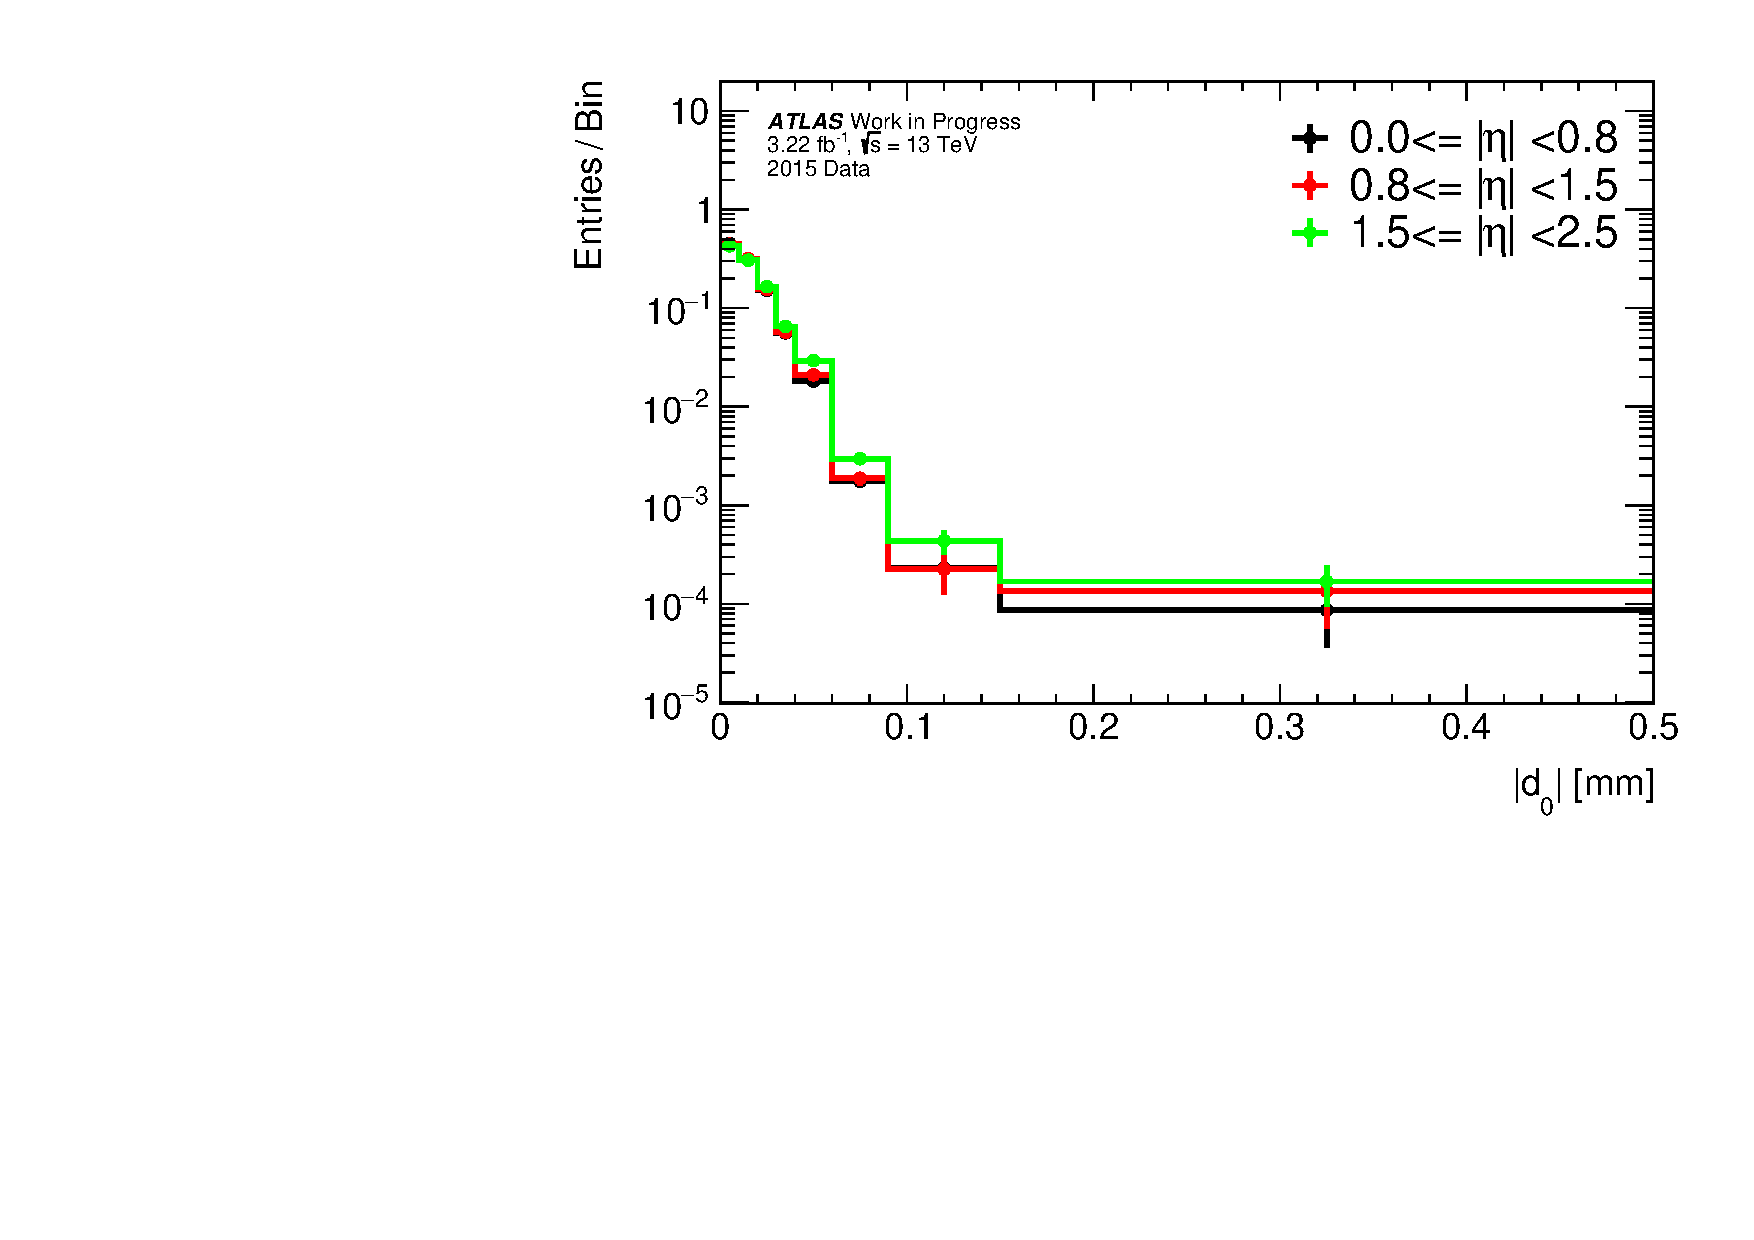
\includegraphics[width=0.45\textwidth]{figures/ZR/d0_smearing/twoplots_TwoPlots_eta-fit_fabs_lep_0_trk_d0_cor-ZR-mu.pdf}
\caption{
  Normalised $d_0$ distributions in data of muons with $0 < |\eta| < 0.8$, $0.8 < |\eta| < 1.5$ and $1.5 < |\eta| < 2.5$. 
  For all distributions muons with $30 < p_T < 35$ GeV were used.
  Signal region (left) and $Z^{0}\rightarrow\mu^{+}\mu^{-}$ region (right).
}
\label{fig:d0_2015_etaDep}
\end{figure}

The whole $p_T$ range is divided into \todo{8 bins}.
The $|\eta|$ range is divided into three bins.
The details of these divisions are given in Tables~\ref{tbl:def_kinematicBinning_pT} and \ref{tbl:def_kinematicBinning_eta}.
By definition, the kinematic bin $i$ $j$ contains all muons with $p_T$ in bin $i$ and $|\eta|$ in bin $j$.
Thus, we define \todo{24} kinematic bins in total.
A considerable number of events in the selected calibration samples ensures that appropriate statistics is available in each bin.

\begin{table}[h]
\begin{center}
 \begin{tabular}{ c | c | c | c } 
 \hline
 $p_T$ bin number ($n_{p_T}$) & $p_T$ range (GeV) & $p_T$ bin number ($n_{p_T}$) & $p_T$ range (GeV) \\
 \hline
%  [27,30,35,40,45,50,65,80,250]
 0 & 27 - 30 & 5 & 50 - 65 \\
 1 & 30 - 35 & 6 & 65 - 80 \\
 2 & 35 - 40 & 7 & 80 - 250\\
 3 & 40 - 45 & & \\ % > 250??
 4 & 45 - 50 & & \\
 \hline
\end{tabular}
\caption{
    Definition of $p_T$ bins.
}%
\label{tbl:def_kinematicBinning_pT}
\end{center}
\end{table}

\begin{table}[h]
\begin{center}
 \begin{tabular}{ c | c  } 
 \hline
 $\eta$ bin number ($n_{\eta}$) & $\eta$ range \\
 \hline
%  [0, 0.8, 1.5, 2.5]
0 & 0 - 0.8 \\
1 & 0.8 - 1.5 \\
2 & 1.5 - 2.5 \\
 \hline
\end{tabular}
\caption{
    Definition of $\eta$ bins.
}%
\label{tbl:def_kinematicBinning_eta}
\end{center}
\end{table}

% To determine the impact of the difference in the $d_0$ resolution between data and MC on the $d_0$ distribution of $W \rightarrow \ell$, where $\ell = e, \mu$.
The resolution is determined by the fit to the $d_0$ distribution of muons in a sample selected in leptonic Z region. 
This sample contains mainly prompt leptons as demonstrated in Fig.\ref{fig:Zmumu_mass_composition}.
The fit is performed in each kinematic bin in the $d_0$ range between $\pm2\dot\sigma$.
% \todo{between $-0.02$ and $0.02$ mm}. 
We use a Gaussian with mean floating around zero as a fitting function.
An example of the fit for muons with $30 < p_T < 35$ GeV and $|\eta| < 0.8$ is shown in Fig.~\ref{fig:d0_2015_fitexample}.
The distribution of the $d_0$ resolution includes also the non-Gaussian tails.
% However, the Gaussian part contains significant fraction of all leptons.
% Moreover, the corrections to the $d_0$ templates due to the differences between data and MC are found to be at the level of ∼ 1\%, as shown in Fig. 23. 
Hence, using just a Gaussian part of the $d_0$ resolution is sufficient for this study.

\begin{figure}[htbp]
\centering
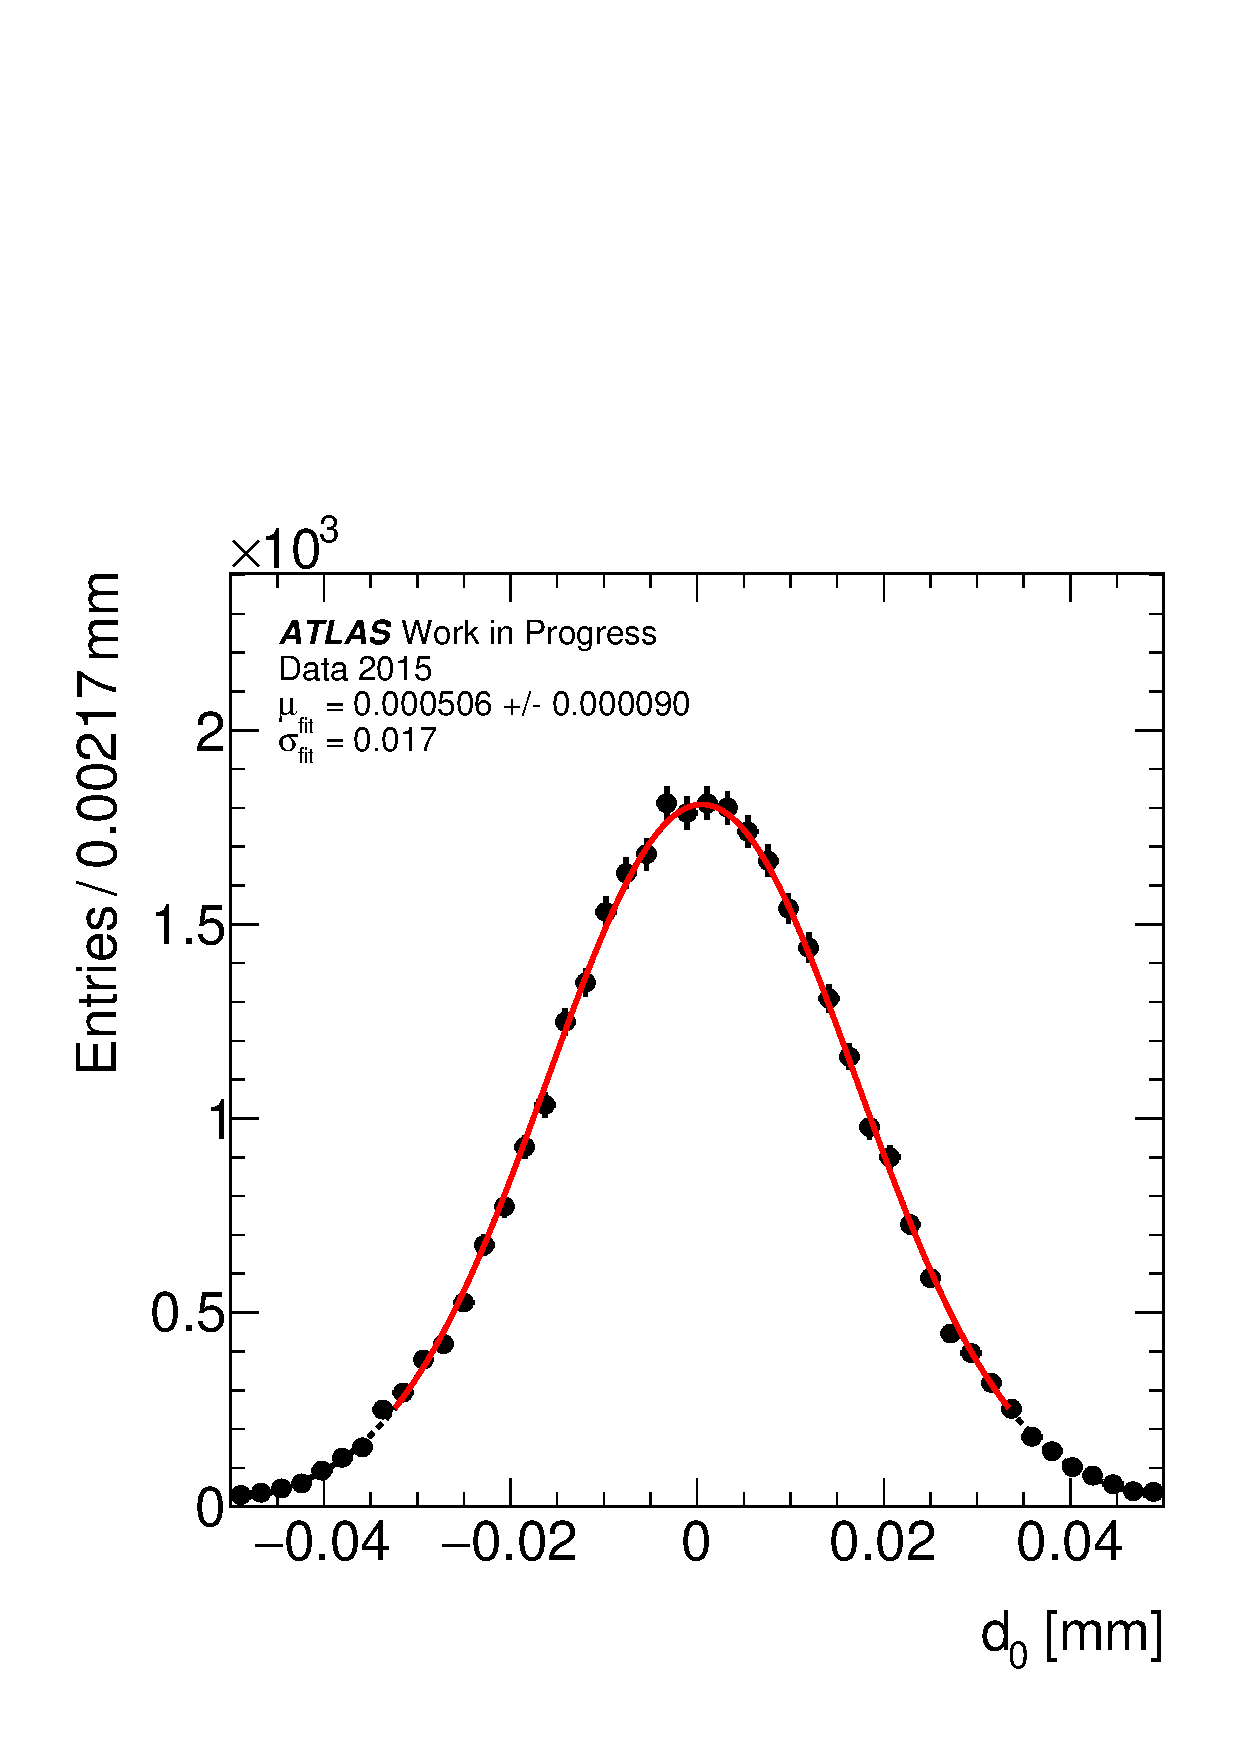
\includegraphics[width=0.55\textwidth]{figures/ZR/d0_smearing/fitDebug_lep_0_trk_d0_cor_kineticBinsResoFit-ZR_etaKinematicBinning_from_0p0_to_0p8_ptKinematicBinning_from_30p0_to_35p0_bin1-mu-Data.pdf}
\caption{
  The $d_0$ distribution of probe muons with $30 < p_T < 35$ GeV and $|\eta| < 0.8$ in the 2015 sample. 
  The full curve shows the fit of this distribution in the range $\pm2\dot\sigma$ by a Gaussian function. 
  The dashed curve shows the extrapolation of this curve beyond the fit range.
}
\label{fig:d0_2015_fitexample}
\end{figure}

The $d_0$ resolution of muons contained in different kinematic bins is shown in Fig.~\ref{fig:d0_resolution}.
In this figure, the kinematic bin number ($n_k$) for the kinematic bin $ij$ is defined as \todo{$n_k = i + 8\dot j$}.
The resolution in Monte Carlo is better than in data.
This effect is increased in the bins with high $p_T$ of the leading lepton.
% We also notice that the resolution is worse in 2015-2016 and is the best in the 2018 sample.

\begin{figure}[htbp]
\centering
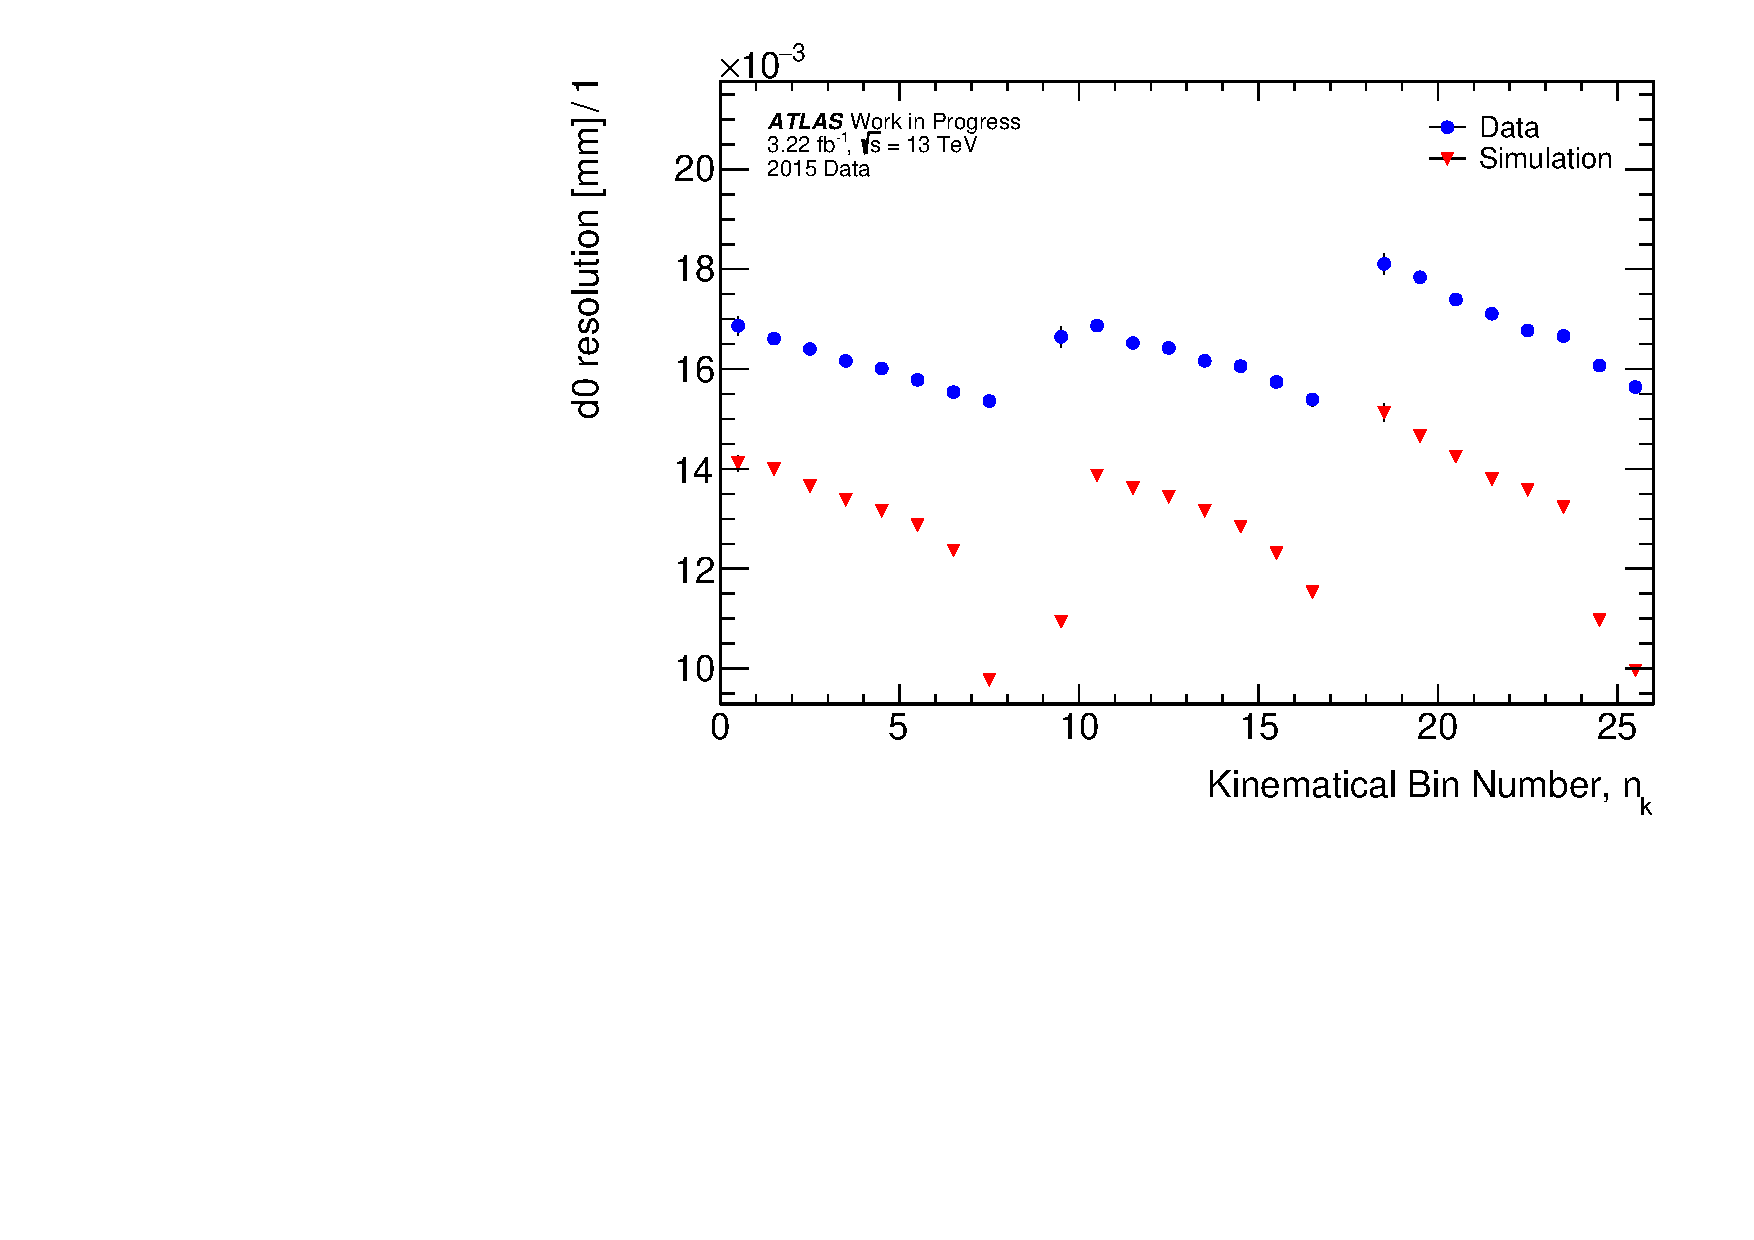
\includegraphics[width=0.65\textwidth]{figures/ZR/d0_smearing/kinematic_lep_0_trk_d0_kineticBinsResoFit-ZR-mu.pdf} %2015
% \\
% 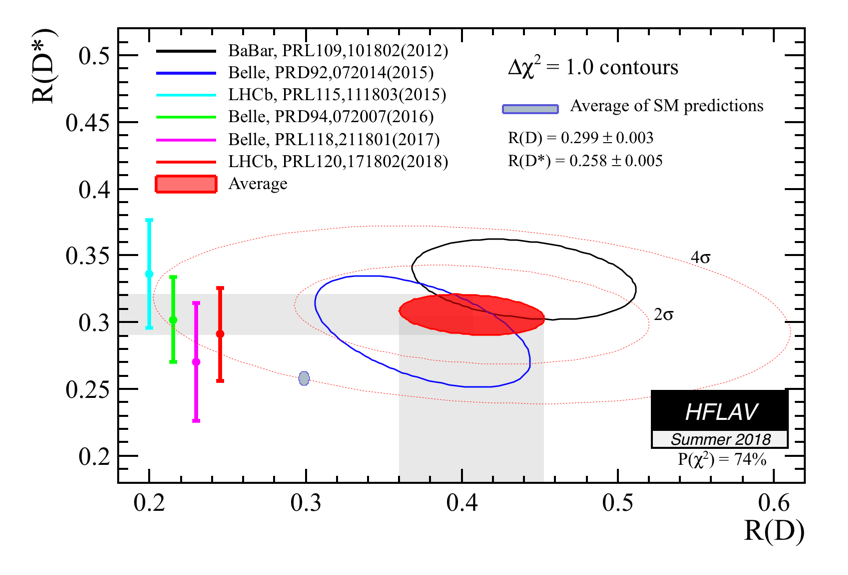
\includegraphics[width=0.65\textwidth]{figures/intro/rdrds_summer18.png} %2016
% \\
% 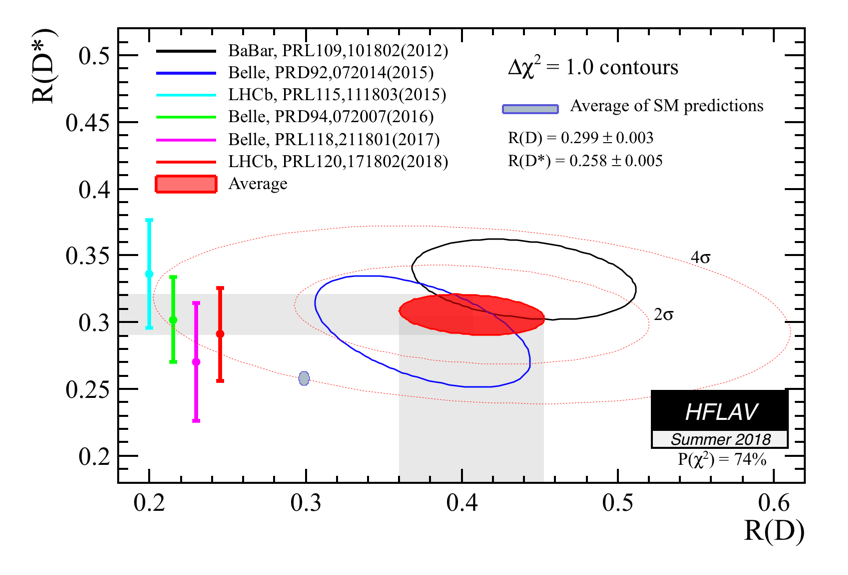
\includegraphics[width=0.65\textwidth]{figures/intro/rdrds_summer18.png} %2017
% \\
% 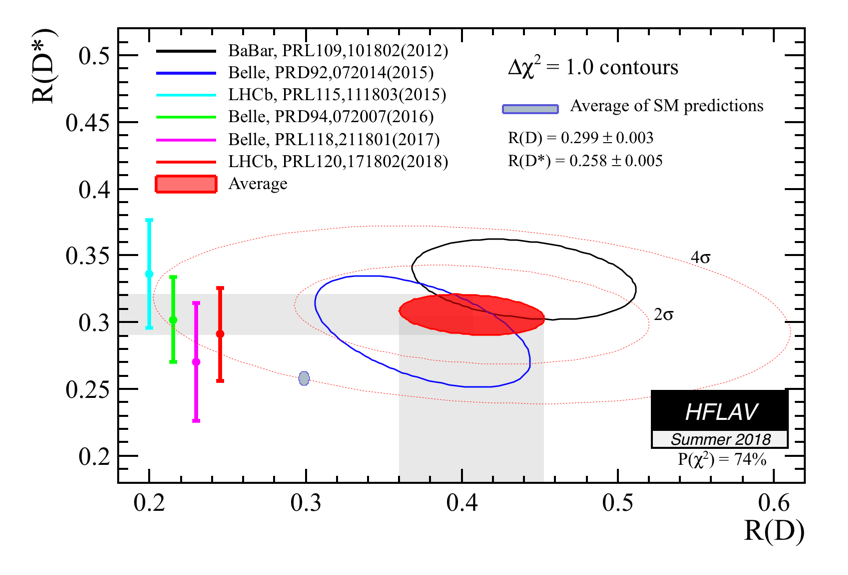
\includegraphics[width=0.65\textwidth]{figures/intro/rdrds_summer18.png} %2018
\caption{
  The muon $d_0$ resolution for different kinematic bins. 
  The kinematic bin number ($n_k$) for the kinematic bin $ij$ is defined as \todo{$n_k = i + 8\dot j$}.
}
\label{fig:d0_resolution}
\end{figure}

The difference in $d_0$ resolution between data and MC must be taken into account in the $d_0$ templates for $W \rightarrow \ell$, where $\ell = e, \mu$.
We obtain the corrected $d_0$ distributions, $F^{ell}_{ij}(d_0)$, in each kinematic bin $ij$ using the following procedure.
In each MC event, on per event basis we smear the value of $d_0$ of the leptons by a Gaussian defined as:
\begin{equation}
  \label{eq:d0_smearing}
  F^{\ell}(d_{0}) = \sum^{7}_{i=0} \sum^{2}_{j=0} \left( \bar{d_0}_{ij}(MC) + (d_{0} - \bar{d_0}_{ij}(MC)) * \frac{\sigma_{ij}(RD)}{\sigma_{ij}(MC)} \right)
\end{equation}
where $\bar{d_0}_{ij}(MC)$ stands for mean value of $d_0$ distribution in Monte Carlo for the given kinematic bin $ij$ and the values of $\sigma_{ij}(RD)$ and $\sigma_{ij}(MC)$ are shown in Fig.~\ref{fig:d0_resolution}.

% The resulting corrections to the $F^{ell}(d_0)$ distributions due to the $d_0$ resolution is relatively small as it can be inferred from Fig.~\ref{fig:d0_correctionRatio_promt_mu}. 
% This figure shows the ratio of corrected and uncorrected $F^{\ell}(d_0)$ distribution.
% The variation for different values of $d_0$ is of the order \todo{of 15\%}.

% \begin{figure}[htbp]
% \centering
% 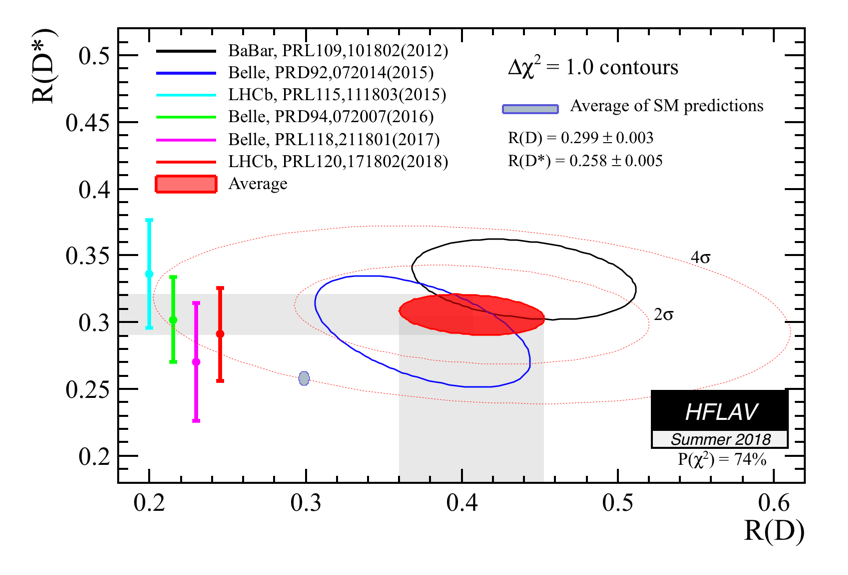
\includegraphics[width=0.65\textwidth]{figures/intro/rdrds_summer18.png} %2015
% % \\
% % 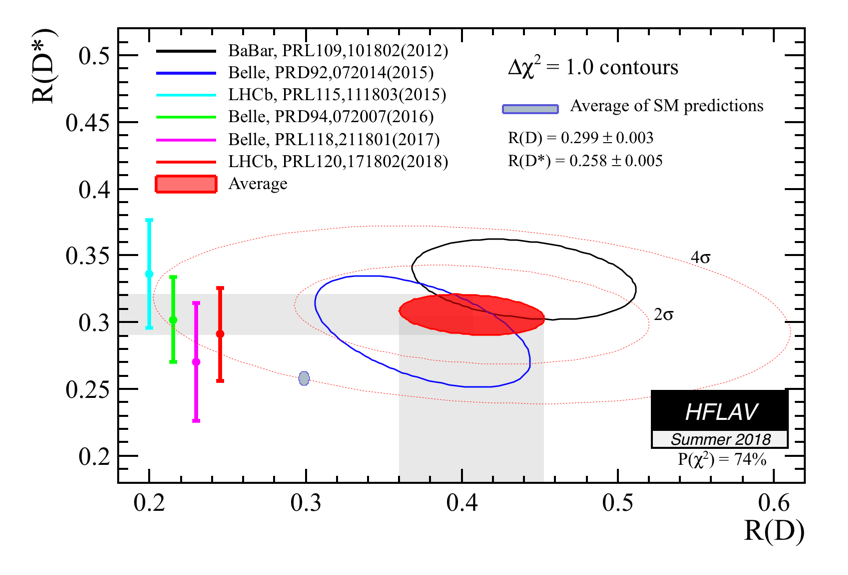
\includegraphics[width=0.65\textwidth]{figures/intro/rdrds_summer18.png} %2016
% % \\
% % 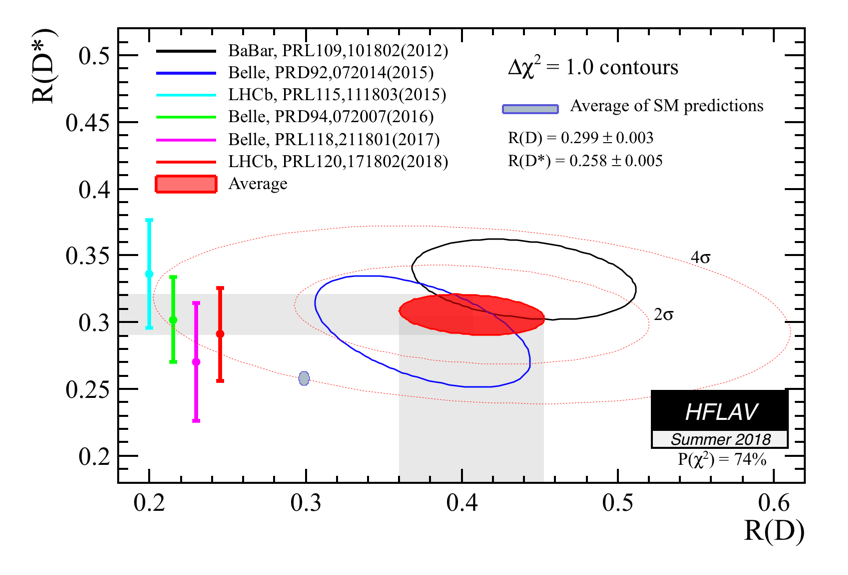
\includegraphics[width=0.65\textwidth]{figures/intro/rdrds_summer18.png} %2017
% % \\
% % 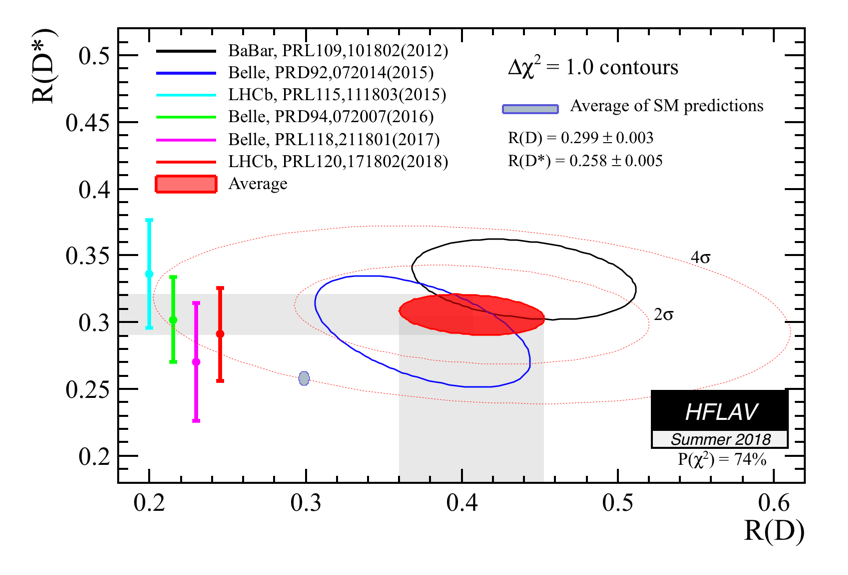
\includegraphics[width=0.65\textwidth]{figures/intro/rdrds_summer18.png} %2018
% \caption{
%   The ratio of corrected and uncorrected $F^{\ell}(d_0)$ distribution for \todo{$W \rightarrow \mu$}.
% }
% \label{fig:d0_correctionRatio_promt_mu}
% \end{figure}

\subsubsection{Impact parameter of muons produced in $\tau$-lepton decays}
\label{sec:d0calibration_of_tau_muons}

The distribution of d0 of muons produced in tauon decays (and denoted as $\tau \rightarrow \ell$, where $\ell = e, \mu$) is taken from Monte Carlo.
Therefore, the description of this variable in simulation must be tested.
This task is performed using the sample enriched in the $Z^{0}\rightarrow\tau^{+}\tau^{-}$ leptonic events.
To obtain this sample we require:
\begin{itemize}
\item one electron and one muon in the event;
\item the charges of the two leptons must be opposite;
\item \todo{$m(e\mu) < 85$} GeV
\item \todo{$p_{T}^{probe} > 15$} GeV
\end{itemize}

\todo{Show that we model Ztautau process well.}

\todo{Show that $d_0$ modelling in Ztautau match/not match data.}

\todo{If not match data, explain how we plan to apply corrections.}



\subsubsection{Impact parameter of fake muons}
\label{sec:d0calibration_of_fake_muons}

In this analysis we obtain fakes by fake factor method. 
The $d_0$ distribution of fake muons is taken from Data, after subtraction corrected MC events from the fake template region.



